%intra.tex
%Par Guillaume Lahaie
%LAHG04077707
%
%%%%%%%%%%%%%%%%%%%%%%%%%%%%%%%%%%%%%%%%%
% Simple Sectioned Essay Template
% LaTeX Template
%
% This template has been downloaded from:
% http://www.latextemplates.com
%
% Note:
% The \lipsum[#] commands throughout this template generate dummy text
% to fill the template out. These commands should all be removed when 
% writing essay content.
%
%%%%%%%%%%%%%%%%%%%%%%%%%%%%%%%%%%%%%%%%%

%----------------------------------------------------------------------------------------
%	PACKAGES AND OTHER DOCUMENT CONFIGURATIONS
%----------------------------------------------------------------------------------------

\documentclass[10.9pt]{article} % Default font size is 12pt, it can be changed here
\renewcommand{\familydefault}{\rmdefault}
\renewcommand{\thesubsection}{\alph{subsection}}

%Pour l'encodage avec accents
\usepackage[utf8]{inputenc}
\usepackage{longtable}
\usepackage{sidecap}

%\usepackage{helvet}
%\renewcommand{\familydefault}{\sfdefault}

\usepackage{afterpage}
\usepackage{appendix}
\usepackage{graphicx} % Required for including pictures
\usepackage{listings}
\usepackage{seqsplit}

\usepackage[left=2.2cm,top=2.2cm,right=2.2cm,bottom=2.2cm,nohead]{geometry} % Required to change the page size to A4
\geometry{letterpaper} % Set the page size to be A4 as opposed to the default US Letter

\usepackage{float} % Allows putting an [H] in \begin{figure} to specify the exact location of the figure
\usepackage{wrapfig} % Allows in-line images such as the example fish picture


\linespread{1.2} % Line spacing

%\setlength\parindent{0pt} % Uncomment to remove all indentation from paragraphs

\graphicspath{{./Pictures/}} % Specifies the directory where pictures are stored
\usepackage[french,english]{babel}

%Comportement d'un paragraphe
\setlength{\parskip}{\baselineskip}%
\setlength{\parindent}{0pt}%

%Widows/orphans
\widowpenalty10000
\clubpenalty10000

\usepackage[hidelinks]{hyperref}

%Meta-info
\title{INF4500 - examen intra}
\author{Guillaume Lahaie}
\date{Remise: 9 décembre 2013}

\hypersetup{
  pdftitle={INF4500 - examen intra},
  pdfauthor={Guillaume Lahaie}
}

\newcommand\blankpage{%
  \null
  \thispagestyle{empty}%
  \addtocounter{page}{-1}%
  \newpage}

\begin{document}
\selectlanguage{french}
\fussy

%----------------------------------------------------------------------------------------
%	TITLE PAGE
%----------------------------------------------------------------------------------------

\begin{titlepage}

\newcommand{\HRule}{\rule{\linewidth}{0.5mm}} % Defines a new command for the horizontal lines, change thickness here

\center % Center everything on the page

\textsc{\LARGE Université du Québec à Montréal}\\[1.5cm] % Name of your university/college
\textsc{\Large INF4500}\\[0.5cm] % Major heading such as course name

\HRule \\[1.5cm]
{ \huge \bfseries Examen intra}\\[0.4cm] % Title of your document
\HRule \\[1.5cm]

\begin{minipage}{0.4\textwidth}
\begin{flushleft} \large
\emph{Par:}\\
Guillaume Lahaie \\ LAHG04077707 % Your name
\end{flushleft}
\end{minipage}
~
\begin{minipage}{0.4\textwidth}
\begin{flushright} \large
\emph{Remis à:} \\
Abdoulaye Baniré Diallo % Supervisor's Name
\end{flushright}
\end{minipage}\\[4cm]

{\large \emph{Date de remise:} \\ Le 9 décembre 2013}\\[3cm] % Date, change the \today to a set date if you want to be precise

%\includegraphics{Logo}\\[1cm] % Include a department/university logo - this will require the graphicx package

\vfill % Fill the rest of the page with whitespace

\end{titlepage}
\blankpage

%----------------------------------------------------------------------------------------
%	TABLE OF CONTENTS
%----------------------------------------------------------------------------------------

\tableofcontents % Include a table of contents

\newpage % Begins the essay on a new page instead of on the same page as the table of contents 

%----------------------------------------------------------------------------------------
% SECTIONS DU DOCUMENT
%----------------------------------------------------------------------------------------

\section{Introduction}

Le but de ce travail est d'annoter des contigs du génome du blé. Nous n'avons pas d'information concernant
la provenance de ces contigs, ou même l'espèce exacte de provenance. Afin de pouvoir fournir une information 
pertinente, j'ai tout d'abord recherché ce qui est connu concernant le génome du blé.

J'ai tout d'abord cherché à connaitre l'état d'avancement des travaux de séquençage du blé. Pour ce faire, j'ai consulté
la base de données des génomes de NCBI \cite{Triticum eastivum Genome}. On y apprend des informations de base sur le
génome du blé. On y apprend que le génome du blé a une taille de 16000 Mb distribué en 21 chromosomes. De plus, les chromosomes
ont une forme allohexaploid composée de trois sous-génomes. La nature hexaploid de son génome a ralenti les efforts de séquençage.

Une première référence de génome du blé a été créée avec l'espèce Triticum urartu \cite{Triticum urartu}. Ce génome est toutefois
celui d'un progéniteur du Triticum aestivum, il peut être utile pour aider à améliorer le génome du blé.

On peut obtenir une information plus complète concernant l'avancement du séquençage du Triticum aestivum sur le site du International
Wheat Genome Sequencing Consortium. On y retrouve deux projets parallèles: en premier lieu, un projet de survey sequencing, afin de
produire un contenu de gène potentiel et un ordre de gène virtuel \cite{IWGSC-survey}. Un autre projet en cours est de produire une
séquence de référence pour le génome du Triticum aestivum \cite{IWGSC-reference}. Ce projet semble être à ses débuts, car il semble
être en cours d'obtention de financement.

D'autres bases de données offrent de l'information à propos du génome du blé, par exemple CerealsDB \cite{cerealsDB}, ayant un génome
de travail du blé. Il y a aussi beaucoup d'autres projets, considérant la place importante occupée par le blé dans l'agriculture moderne.

Basé sur ces informations, j'ai décidé de concentrer mes recherches pour l'annotation des contigs fournis sur les données déjà
connues du génome du blé. Je vais donc seulement garder les résultats de Blast provenant du Triticum aestivum. Bien sûr, il s'agit
ici d'une première étape de recherche, il serait ensuite possible d'élargir la recherche pour identifier des zones fonctionnelles possibles
des contigs, ce qui ne sera pas fait dans ce travail.

Avant de commencer le travail d'annotation, j'ai d'abord jeté un coup sur les informations de qualité des contigs donnés. Pour la majorité
des contigs, la qualité est assez basse, avec des scores autour de 10 à 15. Cela pourrait s'expliquer par la longueur de ces contigs.
Quoi qu'il en soit, c'est une information à retenir tout au long du travail.


\newpage
\section{Produisez une analyse sommaire de ces contigs en présentant la distribution des tailles et taux de GC} % Major section

Afin de compiler et de représenter la taille et le taux de GC des contigs produits par
CAP3, j'ai écrit un script python (question1.py) permettant d'extraire les informations du
fichier seq.data.cap.contigs. Le fichier contient 346 contigs.

Le script produit deux types de graphiques, à l'aide de gnuplot. Le premier type est un
histogramme, un pour la taille des contigs, et un pour le taux de GC des contigs. On peut
alors remarquer la distribution de ces valeurs. Voici les deux histogrammes:
\begin{figure}[p]
\centering
\includegraphics[scale=0.6,angle=270]{question_1/histogramme_taille.eps}
\caption{Histogramme de la taille des contigs}
\includegraphics[scale=0.6,angle=270]{question_1/histogramme_taux.eps}
\caption{Histogramme du taux de GC des contigs}
\end{figure}

J'ai ensuite produit deux graphiques permettant de visualiser différemment ces résultats. On peut
y retrouver la moyenne de taille, la moyenne de taux de GC, ainsi que les contigs se situant en
haut ou en bas ce cette moyenne. On peut aussi voir les valeurs exactes dans le tableau en annexe \ref{1}

La taille moyenne des 346 contigs est de 109 nucléotides, avec un taux de GC moyen de 42,96\%. Ce taux semble
indiquer une prépondérance de région non-codante dans les contigs, car généralement les séquences codantes ont
un taux de GC supérieur aux séquences non-codantes \cite{Wikipedia-GC}.

\begin{figure}[p]
\centering
\includegraphics[scale=0.6,angle=270]{question_1/contigs_taille.eps}
\caption{Nuage de points de la taille des contigs}
\includegraphics[scale=0.6,angle=270]{question_1/contigs_taux.eps}
\caption{Nuage de points du taux de GC des contigs}
\end{figure}


%----------------------------------------------------------------------------------------
% SECTIONS DU DOCUMENT
%----------------------------------------------------------------------------------------
\newpage
\section{Identifiez les annotations Genbank de ces contigs et présentez les dans une table contenant
les colonnes: contigs, numéros Accession, description, uniref id} % Major section

\subsection{Numéros d'accessions et description}
Pour trouver les annotations Genbank des contigs, j'ai tout d'abord effectué un blast de chaque contig
sur la base de données nr/nt de NCBI \cite{BLAST}. J'ai utilisé le script biopython question2.py pour
effectuer tous les blasts, et enregistrer les résultats.

En examinant les résultats de façon sommaire, on remarque une très grande différence entre la qualité des
résultats. Certains ont des E-value très haute, alors que certains ont des valeurs indiquant un résultat de
haute qualité. On peut s'attendre à cela, considérant la grande variabilité des contigs.

Pour traiter les contigs selon leur taille, je calcule la valeur médiane des E-value pour les contigs plus
petits que la taille moyenne. Je fais le même exercice pour les contigs plus grands que la moyenne. Pour
le moment, je m'intéresse au meilleur résultat obtenu seulement pour la médiane.

Comme mentionné en introduction, comme cette analyse s'intéresse seulement au contigs ayant des résultats
pour le Triticum, je ne considère pas dans mes résultats les valeurs de blast pour des espèces différentes
du blé. Je prends donc, dans les résultats de blast, le premier correspondant à un match avec le blé.

J'ai enregistré les résultats dans les fichiers evalue\_lower.txt et evalue\_higher.txt, à l'aide du script
q2\_meanEvalue.py. On peut remarquer que la grande majorité des résultats  obtenus ont des E-values de bonne
qualité, avec un ordre de grandeur permettant d'avoir une grande confiance dans le hit. Basé sur ces données,
je garderai donc tous les résultats, peu importe la taille du contig, ayant une E-value plus petite que 0.01.

Afin d'obtenir les données de numéro d'accession, j'ai modifié le script précédent pour créer un fichier associant
le numéro du contig avec le hit gardé (pour le moment, je garde seulement le premier hit de blé du résultat), avec
le numéro d'accession et la description du hit. Ces données sont gardées seulement si le hit correspond aux
exigences de E-value et de description de hit.

\subsection{Uniref}

Pour obtenir un Uniref \cite{Uniref} pour les contigs retenus, j'ai ensuite utilisé le module bioservices de python permettant
de se connecter au service idmapping de uniprot, pour trouver les identifiants uniref des contigs conservés.

Des 223 contigs restant, 113 ont obtenu des résultats de mapping. Avant de sortir les résultats, j'ai vérifié
le format des données obtenues par ce mapping. Pour certains contigs, un seul résultat est obtenu, alors que
pour certains, on obtient plusieurs mappings différents. Les fichiers XML ne comprennent aucune information
concernant le meilleur résultat, toutefois le service REST utilisé pour le mapping demande de trier les
résultats selon le meilleur score.

Afin de vérifier le résultat, j'ai tenté de blaster un des contigs directement sur la base de données Uniref100,
sur le site \url{http://www.uniprot.org}. Le résultat a été surprenant. J'ai utilisé le contig 2 comme essai,
et le blastx sur Uniref100 n'a retourné aucun hit. Afin de confirmer ce résultat, j'ai effectué le même blastx
en utilisant le service d'EBI et en blastant sur toutes les bases de données de protéines de uniprot. J'ai obtenu
le même résultat.

Je crois que ce résutat est dû au mécanisme de mapping. Comme nous avons pu le constater à la questions 1,
la plupart des contigs donnés ont une longueur moyenne de 109 nucléotides. Toutefois, le numéro d'accession
donnée pour effectuer le id mapping peut correspondre à une très longue séquence. C'est le cas du numéro
d'accession pour le contig 2, il s'agit en fait d'un chromosome complet du blé, ce qui explique les nombreux
résultats du mapping.

J'ai donc décidé de procéder différemment pour obtenir les identifiants uniref correspondant spécifiquement au contig.
J'ai effectué un blastx directement sur la base de données uniref100 pour chaque contig. Pour ce faire, j'ai utilisé
le script q2\_ebi.py. Encore une fois, j'ai utilisé le module bioservices de python pour cette tâche.

J'ai ensuite vérifier les résultats des blasts pour les contigs retenus précédemment. J'ai appliqué le même
filtre: je vérifie tout d'abord si la description du résultat est pour le blé, et ensuite si le E-value 
correspond à une valeur acceptable. Je prends la même valeur que pour les numéros d'accession genbank: 0.01.

Après avoir appliqué ce filtre, il me reste 70 contigs pour lesquels j'ai un numéro d'accession genbank et
un numéro uniref.

\subsection{Construction du tableau}

Comme j'utilise latex pour la rédaction de mon rapport, j'ai écrit un script afin de combiner les informations
de mes différents scripts dans un tableau que je peux insérer directement dans mon fichier latex (q2\_tableau.py).

Le tableau créé rassemble les informations des 223 contigs ayant un résultat de blast pour le blé. Les informations
pour les autres contigs n'est pas présenté. Pour ces contigs, j'indique aussi le uniref trouvé, si une valeur
correspondante existe.

\begingroup
\footnotesize{
\begin{longtable}{|p{1.5cm}|p{2cm}|p{9cm}|p{3cm}|}
\hline
\centering{\bf{Contig}} &\centering{\bf{Accession}} &\centering{\bf{Description}} &\centering{\bf{Uniref - EBI}}\\
\endhead\hline
2 & FN564434 & Triticum aestivum chromosome 3B-specific BAC library, contig ctg0954b. & \\
\hline
3 & EF109232 & Triticum aestivum strain CRB-INRA-CFD-13471 malate dehydrogenase (Mdh4B) gene, partial cds. & \\
\hline
4 & FN564434 & Triticum aestivum chromosome 3B-specific BAC library, contig ctg0954b. & \\
\hline
5 & AK331959 & Triticum aestivum cDNA, clone: WT002\_M17, cultivar: Chinese Spring. & UniRef100\_M7YGL9\\
\hline
6 & AK332278 & Triticum aestivum cDNA, clone: WT003\_J14, cultivar: Chinese Spring. & \\
\hline
7 & AK335464 & Triticum aestivum cDNA, clone: WT012\_P12, cultivar: Chinese Spring. & \\
\hline
10 & JQ240472 & Triticum urartu clones BAC 70G09, BAC 169L13, and BAC 78P09, complete sequence. & \\
\hline
14 & AK332744 & Triticum aestivum cDNA, clone: WT004\_M05, cultivar: Chinese Spring. & \\
\hline
16 & AK332362 & Triticum aestivum cDNA, clone: WT003\_M19, cultivar: Chinese Spring. & \\
\hline
18 & U73217 & Triticum aestivum cold acclimation protein WCOR615 (Wcor615) mRNA, complete cds. & \\
\hline
21 & DQ286562 & Triticum aestivum putative lipid transfer protein mRNA, complete cds. & \\
\hline
22 & KC816724 & Triticum urartu cultivar G1812 clone BAC 288D18 chromosome 3AL, complete sequence. & \\
\hline
23 & AK335482 & Triticum aestivum cDNA, clone: WT013\_A03, cultivar: Chinese Spring. & \\
\hline
24 & AK330641 & Triticum aestivum cDNA, clone: SET4\_P05, cultivar: Chinese Spring. & UniRef100\_M8ABV0\\
\hline
25 & AK331680 & Triticum aestivum cDNA, clone: SET1\_K05, cultivar: Chinese Spring. & \\
\hline
26 & AK332086 & Triticum aestivum cDNA, clone: WT003\_B19, cultivar: Chinese Spring. & UniRef100\_M7YAN9\\
\hline
27 & EU660894 & Triticum turgidum subsp. durum clone BAC 1053F12+1054I5 cytosolic acetyl-CoA carboxylase (Acc-2) and putative amino acid permease genes, complete cds. & \\
\hline
29 & BT008986 & Triticum aestivum clone wdk2c.pk008.b17:fis, full insert mRNA sequence. & \\
\hline
30 & HQ596874 & Triticum aestivum voucher AP212 trnH-psbA intergenic spacer, partial sequence; chloroplast. & \\
\hline
31 & HQ391280 & Triticum aestivum clone UCDTA01731 genomic sequence. & UniRef100\_M8A3H2\\
\hline
33 & HE996560 & Triticum aestivum cv. Arina SNP, chromosome 3B, clone Taes\_arina\_ctg\_58725. & UniRef100\_D9CJA9\\
\hline
34 & HQ391329 & Triticum aestivum clone UCDTA01780 genomic sequence. & \\
\hline
35 & EU159424 & Triticum turgidum haplotype B DNA repair protein Rad50 gene, complete cds. & \\
\hline
36 & DQ251490 & Triticum aestivum cultivar Chinese Spring powdery mildew resistance protein PM3CS (Pm3) gene, Pm3-CS allele, complete cds. & \\
\hline
37 & KC290909 & Triticum aestivum clone pTa-s309 FISH-positive repetitive sequence. & UniRef100\_T1L6W5\\
\hline
39 & AJ318783 & Triticum sp. partial mRNA for replication factor C, large subunit (rfc-1 gene). & UniRef100\_Q8L6A5\\
\hline
40 & AK330233 & Triticum aestivum cDNA, clone: SET3\_P11, cultivar: Chinese Spring. & UniRef100\_T1N886\\
\hline
41 & FN564434 & Triticum aestivum chromosome 3B-specific BAC library, contig ctg0954b. & \\
\hline
44 & AJ784900 & Triticum aestivum mRNA for type 1 non-specific lipid transfer protein precursor (ltp9.4 gene). & \\
\hline
46 & AK330669 & Triticum aestivum cDNA, clone: SET1\_G08, cultivar: Chinese Spring. & \\
\hline
47 & AK331428 & Triticum aestivum cDNA, clone: WT007\_H14, cultivar: Chinese Spring. & UniRef100\_M8AEN7\\
\hline
48 & HE996767 & Triticum aestivum cv. Arina SNP, chromosome 3B, clone Taes\_arina\_ctg\_66371. & UniRef100\_M7Z3W8\\
\hline
49 & AK332525 & Triticum aestivum cDNA, clone: SET1\_N11, cultivar: Chinese Spring. & \\
\hline
51 & AK331813 & Triticum aestivum cDNA, clone: WT002\_G19, cultivar: Chinese Spring. & \\
\hline
53 & HE996642 & Triticum aestivum cv. Arina SNP, chromosome 3B, clone Taes\_arina\_ctg\_60579. & UniRef100\_T1M429\\
\hline
56 & HQ390245 & Triticum turgidum clone UCDTA00696 genomic sequence. & \\
\hline
57 & FJ345689 & Triticum aestivum MITE Tourist-3 MITE Islay Tourist, complete sequence. & \\
\hline
58 & JF758499 & Triticum aestivum clone BAC 425P7, complete sequence. & UniRef100\_M7Z3R4\\
\hline
59 & FN645450 & Triticum aestivum chromosome 3B-specific BAC library, contig ctg0011b. & \\
\hline
60 & FN645450 & Triticum aestivum chromosome 3B-specific BAC library, contig ctg0011b. & \\
\hline
61 & AK333585 & Triticum aestivum cDNA, clone: WT006\_N11, cultivar: Chinese Spring. & UniRef100\_M8A091\\
\hline
63 & FN564428 & Triticum aestivum chromosome 3B-specific BAC library, contig ctg0091b. & \\
\hline
67 & AK332970 & Triticum aestivum cDNA, clone: WT005\_F05, cultivar: Chinese Spring. & UniRef100\_M7YP29\\
\hline
70 & AK332566 & Triticum aestivum cDNA, clone: WT004\_E21, cultivar: Chinese Spring. & \\
\hline
71 & AK334580 & Triticum aestivum cDNA, clone: SET1\_C02, cultivar: Chinese Spring. & \\
\hline
73 & EU660896 & Triticum urartu clone BAC 059G16 plastid acetyl-CoA carboxylase (Acc-1) gene, complete cds; nuclear gene for plastid product. & UniRef100\_M7ZVV5\\
\hline
74 & KC912694 & Triticum aestivum chloroplast, complete genome. & \\
\hline
75 & AB238931 & Triticum monococcum TmABI1 gene for protein phosphatase 2C, complete cds. & UniRef100\_M7YVM1\\
\hline
76 & BT009089 & Triticum aestivum clone wkm2c.pk0002.a3:fis, full insert mRNA sequence. & \\
\hline
78 & AK335897 & Triticum aestivum cDNA, clone: SET2\_L19, cultivar: Chinese Spring. & UniRef100\_M7ZH67\\
\hline
80 & AK330275 & Triticum aestivum cDNA, clone: SET4\_A24, cultivar: Chinese Spring. & \\
\hline
81 & HE996341 & Triticum aestivum cv. Arina SNP, chromosome 3B, clone Taes\_arina\_ctg\_16989. & \\
\hline
84 & JF758499 & Triticum aestivum clone BAC 425P7, complete sequence. & \\
\hline
86 & AK335765 & Triticum aestivum cDNA, clone: WT013\_L14, cultivar: Chinese Spring. & UniRef100\_M7YZ42\\
\hline
88 & FN564432 & Triticum aestivum chromosome 3B-specific BAC library, contig ctg0616b. & \\
\hline
91 & AM932681 & Triticum aestivum 3B chromosome, clone BAC TA3B63B13. & \\
\hline
92 & U76215 & Triticum aestivum NBS-LRR type protein pseudogene, complete sequence. & \\
\hline
94 & HE996549 & Triticum aestivum cv. Arina SNP, chromosome 3B, clone Taes\_arina\_ctg\_58561. & \\
\hline
95 & AY487917 & Triticum aestivum Mla-like protein mRNA, partial cds. & UniRef100\_Q6RW52\\
\hline
96 & KC912694 & Triticum aestivum chloroplast, complete genome. & UniRef100\_T1MEW5\\
\hline
97 & KC912694 & Triticum aestivum chloroplast, complete genome. & \\
\hline
98 & AK333621 & Triticum aestivum cDNA, clone: WT006\_O21, cultivar: Chinese Spring. & \\
\hline
99 & KC912694 & Triticum aestivum chloroplast, complete genome. & \\
\hline
100 & AK333932 & Triticum aestivum cDNA, clone: WT008\_N17, cultivar: Chinese Spring. & UniRef100\_T1N9G3\\
\hline
101 & AK331581 & Triticum aestivum cDNA, clone: SET1\_J20, cultivar: Chinese Spring. & \\
\hline
102 & KC912694 & Triticum aestivum chloroplast, complete genome. & \\
\hline
104 & HQ391318 & Triticum aestivum clone UCDTA01769 genomic sequence. & UniRef100\_T1MZT0\\
\hline
105 & HQ391224 & Triticum aestivum clone UCDTA01675 genomic sequence. & UniRef100\_M7ZMV6\\
\hline
108 & DQ286562 & Triticum aestivum putative lipid transfer protein mRNA, complete cds. & \\
\hline
109 & AK335062 & Triticum aestivum cDNA, clone: WT011\_P12, cultivar: Chinese Spring. & UniRef100\_M7ZAY8\\
\hline
110 & KC152455 & Triticum aestivum clone BAC321B14 MATE1B gene, complete cds. & \\
\hline
112 & AK332529 & Triticum aestivum cDNA, clone: WT004\_D08, cultivar: Chinese Spring. & UniRef100\_M7ZA56\\
\hline
115 & AY049041 & Triticum aestivum 28S ribosomal RNA gene, partial sequence. & UniRef100\_T1L6Y4\\
\hline
117 & AK334519 & Triticum aestivum cDNA, clone: WT010\_C18, cultivar: Chinese Spring. & \\
\hline
119 & AK333035 & Triticum aestivum cDNA, clone: WT005\_H19, cultivar: Chinese Spring. & UniRef100\_Q9FT38\\
\hline
120 & CT009735 & Triticum aestivum. & \\
\hline
121 & HE996280 & Triticum aestivum cv. Arina SNP, chromosome 3B, clone Taes\_arina\_ctg\_14118. & UniRef100\_M8AZM6\\
\hline
122 & EU626553 & Triticum urartu clone BAC 261N5, complete sequence. & \\
\hline
123 & HQ391007 & Triticum aestivum clone UCDTA01458 genomic sequence. & \\
\hline
125 & KC912694 & Triticum aestivum chloroplast, complete genome. & UniRef100\_T1LKW9\\
\hline
127 & AK330423 & Triticum aestivum cDNA, clone: SET4\_G18, cultivar: Chinese Spring. & UniRef100\_M8AIQ8\\
\hline
131 & HF541875 & Triticum aestivum chromosome 3B specific BAC library, BAC clone TaaCsp3BFhA\_0147D05. & UniRef100\_M7ZGW4\\
\hline
132 & CT009735 & Triticum aestivum. & UniRef100\_T1LKM3\\
\hline
135 & HQ391329 & Triticum aestivum clone UCDTA01780 genomic sequence. & \\
\hline
136 & KC912694 & Triticum aestivum chloroplast, complete genome. & UniRef100\_M7ZC27\\
\hline
137 & AK332255 & Triticum aestivum cDNA, clone: WT003\_I14, cultivar: Chinese Spring. & UniRef100\_M7YN64\\
\hline
144 & AK332897 & Triticum aestivum cDNA, clone: WT005\_C09, cultivar: Chinese Spring. & \\
\hline
146 & EF219468 & Triticum aestivum translationally-controlled tumor protein mRNA, complete cds. & UniRef100\_M7YF70\\
\hline
148 & AJ001117 & Triticum aestivum mRNA for sucrose synthase type I. & \\
\hline
150 & AK330745 & Triticum aestivum cDNA, clone: SET5\_D06, cultivar: Chinese Spring. & UniRef100\_M7YEA6\\
\hline
151 & AK335219 & Triticum aestivum cDNA, clone: WT012\_F19, cultivar: Chinese Spring. & UniRef100\_M7ZDI5\\
\hline
152 & AK335725 & Triticum aestivum cDNA, clone: SET2\_K04, cultivar: Chinese Spring. & UniRef100\_M7ZVF6\\
\hline
153 & BT009622 & Triticum aestivum clone wre1n.pk0137.c12:fis, full insert mRNA sequence. & \\
\hline
154 & HE774675 & Triticum aestivum chromosome arm 3DS-specific BAC library, contig ctg1484. & \\
\hline
157 & FN564428 & Triticum aestivum chromosome 3B-specific BAC library, contig ctg0091b. & \\
\hline
158 & EU626553 & Triticum urartu clone BAC 261N5, complete sequence. & \\
\hline
159 & DQ862833 & Triticum monococcum S-adenosylhomocysteine hydrolase mRNA, partial cds. & \\
\hline
161 & AK330639 & Triticum aestivum cDNA, clone: SET4\_P03, cultivar: Chinese Spring. & \\
\hline
162 & KC912694 & Triticum aestivum chloroplast, complete genome. & UniRef100\_T1LKW9\\
\hline
164 & DQ432014 & Triticum aestivum vacuolar proton-ATPase subunit A mRNA, complete cds. & \\
\hline
165 & KC912694 & Triticum aestivum chloroplast, complete genome. & UniRef100\_T1LKW9\\
\hline
166 & EU835980 & Triticum aestivum clone BAC 502E09, complete sequence. & \\
\hline
167 & FN564426 & Triticum aestivum chromosome 3B-specific BAC library, contig ctg0005b. & \\
\hline
168 & JF439307 & Triticum aestivum cultivar Yang Mai 158 serine/threonine protein kinase Stpk-D (Stpk-D) gene, complete cds. & \\
\hline
171 & KC175605 & Triticum aestivum calcium-dependent protein kinase 3-like 1 mRNA, partial cds. & UniRef100\_M1NQF6\\
\hline
173 & FN564434 & Triticum aestivum chromosome 3B-specific BAC library, contig ctg0954b. & \\
\hline
174 & AK333177 & Triticum aestivum cDNA, clone: WT005\_N11, cultivar: Chinese Spring. & \\
\hline
175 & AJ132439 & Triticum aestivum mRNA for protein encoded by lt1.1 gene, partial. & \\
\hline
176 & AK331581 & Triticum aestivum cDNA, clone: SET1\_J20, cultivar: Chinese Spring. & \\
\hline
177 & HQ390713 & Triticum aestivum clone UCDTA01164 genomic sequence. & \\
\hline
179 & EU660895 & Triticum aestivum clone BAC 1825J10 cytosolic acetyl-CoA carboxylase (Acc-2) and putative amino acid permeases genes, complete cds. & \\
\hline
180 & FN564430 & Triticum aestivum chromosome 3B-specific BAC library, contig ctg0464b. & \\
\hline
181 & FJ427399 & Triticum turgidum clone BAC 738D05 chromosome 4B, partial sequence. & \\
\hline
182 & DQ537336 & Triticum aestivum clones BAC 1289J04; BAC 1001P20, complete sequence. & \\
\hline
184 & AK330153 & Triticum aestivum cDNA, clone: SET3\_M02, cultivar: Chinese Spring. & \\
\hline
185 & JX040632 & Triticum turgidum subsp. durum x Secale cereale glutamine synthetase I (GSI) mRNA, complete cds. & UniRef100\_M7ZP85\\
\hline
187 & AY951945 & Triticum monococcum TmBAC 60J11 FR-Am2 locus, genomic sequence. & \\
\hline
193 & AK332664 & Triticum aestivum cDNA, clone: WT004\_I22, cultivar: Chinese Spring. & \\
\hline
194 & AK330641 & Triticum aestivum cDNA, clone: SET4\_P05, cultivar: Chinese Spring. & UniRef100\_T1MAM1\\
\hline
195 & HE774676 & Triticum aestivum chromosome arm 3DS-specific BAC library, contig ctg447. & \\
\hline
197 & FN564434 & Triticum aestivum chromosome 3B-specific BAC library, contig ctg0954b. & \\
\hline
198 & AK334078 & Triticum aestivum cDNA, clone: WT009\_E03, cultivar: Chinese Spring. & \\
\hline
199 & AM502900 & Triticum aestivum mRNA for MIKC-type MADS-box transcription factor WM30 (WM30 gene). & \\
\hline
201 & AK331183 & Triticum aestivum cDNA, clone: SET6\_K07, cultivar: Chinese Spring. & \\
\hline
203 & AK331090 & Triticum aestivum cDNA, clone: SET6\_A20, cultivar: Chinese Spring. & \\
\hline
206 & FN564430 & Triticum aestivum chromosome 3B-specific BAC library, contig ctg0464b. & \\
\hline
208 & FJ345689 & Triticum aestivum MITE Tourist-3 MITE Islay Tourist, complete sequence. & \\
\hline
211 & GU817319 & Triticum aestivum clone BAC\_2383A24 chromosome 3B, complete sequence. & \\
\hline
213 & AK333846 & Triticum aestivum cDNA, clone: WT008\_O20, cultivar: Chinese Spring. & UniRef100\_M7YLY4\\
\hline
216 & AP013106 & Triticum timopheevii mitochondrial DNA, complete sequence. & \\
\hline
217 & AK332920 & Triticum aestivum cDNA, clone: WT005\_D07, cultivar: Chinese Spring. & \\
\hline
221 & AK334145 & Triticum aestivum cDNA, clone: WT009\_O11, cultivar: Chinese Spring. & \\
\hline
222 & KC912694 & Triticum aestivum chloroplast, complete genome. & UniRef100\_T1LKW9\\
\hline
224 & GU817319 & Triticum aestivum clone BAC\_2383A24 chromosome 3B, complete sequence. & \\
\hline
225 & FR820619 & Triticum turgidum subsp. durum partial mRNA for td3ITN1 protein. & \\
\hline
226 & AK334286 & Triticum aestivum cDNA, clone: WT009\_F09, cultivar: Chinese Spring. & \\
\hline
227 & AK332238 & Triticum aestivum cDNA, clone: WT003\_H22, cultivar: Chinese Spring. & UniRef100\_M7ZLU3\\
\hline
228 & FN564434 & Triticum aestivum chromosome 3B-specific BAC library, contig ctg0954b. & \\
\hline
229 & HQ391114 & Triticum aestivum clone UCDTA01565 genomic sequence. & \\
\hline
231 & GU211169 & Triticum aestivum clone 09d3 gliadin/avenin-like seed protein mRNA, complete cds. & UniRef100\_D2KFH0\\
\hline
233 & AF532601 & Triticum aestivum multidrug resistance associated protein MRP2 mRNA, complete cds. & UniRef100\_M7ZK96\\
\hline
235 & AF389882 & Triticum aestivum clone PAAC-SCGCA5 AFLP sequence. & UniRef100\_T1LCX9\\
\hline
236 & AK333949 & Triticum aestivum cDNA, clone: WT008\_P23, cultivar: Chinese Spring. & \\
\hline
238 & FN564428 & Triticum aestivum chromosome 3B-specific BAC library, contig ctg0091b. & \\
\hline
239 & FN564434 & Triticum aestivum chromosome 3B-specific BAC library, contig ctg0954b. & \\
\hline
240 & HQ435325 & Triticum aestivum clone BAC 1J9 Tmemb\_185A domain-containing protein (1J9.1), EamA domain-containing protein (1J9.2), and Rht-D1b (Rht-D1b) genes, complete cds, complete sequence. & UniRef100\_M7ZYV2\\
\hline
242 & HQ390774 & Triticum aestivum clone UCDTA01225 genomic sequence. & UniRef100\_M7ZSC0\\
\hline
243 & AK330263 & Triticum aestivum cDNA, clone: SET4\_A13, cultivar: Chinese Spring. & \\
\hline
244 & HQ391044 & Triticum aestivum clone UCDTA01495 genomic sequence. & \\
\hline
245 & FN564430 & Triticum aestivum chromosome 3B-specific BAC library, contig ctg0464b. & \\
\hline
247 & KC912694 & Triticum aestivum chloroplast, complete genome. & \\
\hline
250 & FN564430 & Triticum aestivum chromosome 3B-specific BAC library, contig ctg0464b. & \\
\hline
251 & DQ537335 & Triticum aestivum clones BAC 1031P08; BAC 754K10; BAC 1344C16, complete sequence. & \\
\hline
252 & AK335757 & Triticum aestivum cDNA, clone: WT013\_L07, cultivar: Chinese Spring. & \\
\hline
253 & FJ225148 & Triticum aestivum ferritin 2A gene, complete cds. & \\
\hline
254 & HE774676 & Triticum aestivum chromosome arm 3DS-specific BAC library, contig ctg447. & \\
\hline
255 & AP013106 & Triticum timopheevii mitochondrial DNA, complete sequence. & \\
\hline
256 & FN645450 & Triticum aestivum chromosome 3B-specific BAC library, contig ctg0011b. & \\
\hline
257 & AK332440 & Triticum aestivum cDNA, clone: WT003\_P20, cultivar: Chinese Spring. & \\
\hline
258 & AK333064 & Triticum aestivum cDNA, clone: WT005\_I23, cultivar: Chinese Spring. & \\
\hline
259 & AK332804 & Triticum aestivum cDNA, clone: WT004\_O17, cultivar: Chinese Spring. & \\
\hline
260 & FN645450 & Triticum aestivum chromosome 3B-specific BAC library, contig ctg0011b. & \\
\hline
261 & AK335863 & Triticum aestivum cDNA, clone: WT013\_P13, cultivar: Chinese Spring. & UniRef100\_M7YYG6\\
\hline
262 & AB646974 & Triticum aestivum PRR gene for pseudo-response regulator, complete cds, allele: Ppd-B1a.1. & \\
\hline
263 & GU817319 & Triticum aestivum clone BAC\_2383A24 chromosome 3B, complete sequence. & \\
\hline
264 & AK332413 & Triticum aestivum cDNA, clone: WT003\_O18, cultivar: Chinese Spring. & UniRef100\_M7ZIU6\\
\hline
265 & FJ427399 & Triticum turgidum clone BAC 738D05 chromosome 4B, partial sequence. & \\
\hline
266 & DQ154924 & Triticum turgidum RAB7 (RAB7) gene, exons 1, 2 and partial cds; and delta-1-pyrroline-5-carboxylate dehydrogenase (P5CDH) gene, complete cds. & \\
\hline
267 & FN564433 & Triticum aestivum chromosome 3B-specific BAC library, contig ctg0661b. & \\
\hline
268 & AK334924 & Triticum aestivum cDNA, clone: WT011\_I02, cultivar: Chinese Spring. & \\
\hline
269 & AK334063 & Triticum aestivum cDNA, clone: WT009\_A23, cultivar: Chinese Spring. & UniRef100\_M7YKC3\\
\hline
270 & AY465427 & Triticum turgidum subsp. durum putative C3H2C3 RING-finger protein (6G2) gene, complete cds. & \\
\hline
271 & DQ167201 & Triticum aestivum eukaryotic translation initiation factor 5A1 gene, complete cds. & \\
\hline
274 & FN564434 & Triticum aestivum chromosome 3B-specific BAC library, contig ctg0954b. & \\
\hline
275 & GU817319 & Triticum aestivum clone BAC\_2383A24 chromosome 3B, complete sequence. & \\
\hline
276 & AK330938 & Triticum aestivum cDNA, clone: SET5\_K22, cultivar: Chinese Spring. & UniRef100\_M7ZJN7\\
\hline
277 & GQ409824 & Triticum turgidum subsp. durum cultivar Langdon clone BAC 406B11, complete sequence. & \\
\hline
278 & JF946486 & Triticum aestivum transposon TREP 3040\_Harbinger, complete sequence; pseudo-response regulator (Ppd-B1) gene, Ppd-B1a allele, complete cds; and retrotransposon Gypsy TREP 3457\_Danae, complete sequence. & UniRef100\_M8B455\\
\hline
279 & JF701619 & Triticum aestivum cultivar Chinese Spring clone BAC CS12224M17\_A, complete sequence. & \\
\hline
280 & AK334173 & Triticum aestivum cDNA, clone: WT009\_C16, cultivar: Chinese Spring. & \\
\hline
281 & KF282629 & Triticum aestivum cultivar Chinese Spring clone BAC 351D1 chromosome 4A DELLA protein (Rht-A) gene, complete cds, complete sequence. & \\
\hline
284 & AK332097 & Triticum aestivum cDNA, clone: WT003\_C06, cultivar: Chinese Spring. & \\
\hline
286 & EU626553 & Triticum urartu clone BAC 261N5, complete sequence. & \\
\hline
287 & BT009432 & Triticum aestivum clone wlmk1.pk0037.b8:fis, full insert mRNA sequence. & UniRef100\_M7YEM7\\
\hline
289 & FN564432 & Triticum aestivum chromosome 3B-specific BAC library, contig ctg0616b. & \\
\hline
290 & AK335883 & Triticum aestivum cDNA, clone: SET2\_L04, cultivar: Chinese Spring. & \\
\hline
292 & HE774676 & Triticum aestivum chromosome arm 3DS-specific BAC library, contig ctg447. & \\
\hline
293 & AB238931 & Triticum monococcum TmABI1 gene for protein phosphatase 2C, complete cds. & \\
\hline
294 & JQ269664 & Triticum aestivum cultivar WL 711 betaine aldehyde dehydrogenase-like protein mRNA, partial cds. & UniRef100\_H9NAU5\\
\hline
296 & AK335270 & Triticum aestivum cDNA, clone: WT012\_H16, cultivar: Chinese Spring. & \\
\hline
297 & AY968588 & Triticum aestivum ice recrystallization inhibition protein 1 precursor, mRNA, complete cds. & \\
\hline
300 & AK332508 & Triticum aestivum cDNA, clone: WT004\_C11, cultivar: Chinese Spring. & UniRef100\_M7ZMZ7\\
\hline
301 & DQ537335 & Triticum aestivum clones BAC 1031P08; BAC 754K10; BAC 1344C16, complete sequence. & \\
\hline
302 & KC912694 & Triticum aestivum chloroplast, complete genome. & \\
\hline
303 & GU211251 & Triticum aestivum pyruvate dehydrogenase E1 component alpha subunit (PDHA1) gene, partial cds. & \\
\hline
306 & JF261156 & Triticum monococcum cultivar DV92 Mla1 gene, complete cds. & \\
\hline
307 & AK335953 & Triticum aestivum cDNA, clone: SET1\_C22, cultivar: Chinese Spring. & UniRef100\_M8A0S9\\
\hline
308 & KC912694 & Triticum aestivum chloroplast, complete genome. & \\
\hline
309 & HQ821868 & Triticum aestivum cultivar Jasna glutamate dehydrogenase mRNA, complete cds. & UniRef100\_E9NX12\\
\hline
311 & JF946486 & Triticum aestivum transposon TREP 3040\_Harbinger, complete sequence; pseudo-response regulator (Ppd-B1) gene, Ppd-B1a allele, complete cds; and retrotransposon Gypsy TREP 3457\_Danae, complete sequence. & \\
\hline
312 & AK335209 & Triticum aestivum cDNA, clone: WT012\_F09, cultivar: Chinese Spring. & UniRef100\_Q41591\\
\hline
313 & AK336081 & Triticum aestivum cDNA, clone: SET3\_C24, cultivar: Chinese Spring. & UniRef100\_M7YMK8\\
\hline
314 & AM932685 & Triticum aestivum 3B chromosome, clone BAC TA3B95F5. & \\
\hline
316 & GQ169688 & Triticum aestivum plastid glutamine synthetase 2 (GS2) gene, GS2-D1a allele, complete cds; nuclear gene for plastid product. & \\
\hline
318 & FN564428 & Triticum aestivum chromosome 3B-specific BAC library, contig ctg0091b. & \\
\hline
320 & KC573058 & Triticum monococcum subsp. monococcum cultivar DV92 Sr35 region, genomic sequence. & \\
\hline
321 & HE996762 & Triticum aestivum cv. Arina SNP, chromosome 3B, clone Taes\_arina\_ctg\_66287. & UniRef100\_M8A6Z7\\
\hline
324 & GQ409824 & Triticum turgidum subsp. durum cultivar Langdon clone BAC 406B11, complete sequence. & \\
\hline
326 & KC573058 & Triticum monococcum subsp. monococcum cultivar DV92 Sr35 region, genomic sequence. & UniRef100\_M7Z2V6\\
\hline
327 & BT009452 & Triticum aestivum clone wlmk8.pk0022.f7:fis, full insert mRNA sequence. & \\
\hline
328 & HE774675 & Triticum aestivum chromosome arm 3DS-specific BAC library, contig ctg1484. & \\
\hline
329 & AM502905 & Triticum aestivum mRNA for MIKC-type MADS-box transcription factor WM32B (WM32B gene). & UniRef100\_T1LUM5\\
\hline
330 & AK334989 & Triticum aestivum cDNA, clone: WT011\_L15, cultivar: Chinese Spring. & \\
\hline
333 & FN564434 & Triticum aestivum chromosome 3B-specific BAC library, contig ctg0954b. & \\
\hline
334 & AK333292 & Triticum aestivum cDNA, clone: WT006\_B19, cultivar: Chinese Spring. & UniRef100\_M7ZHG4\\
\hline
336 & BT009004 & Triticum aestivum clone wdk2c.pk018.c16:fis, full insert mRNA sequence. & UniRef100\_Q8S9G0\\
\hline
337 & FN564434 & Triticum aestivum chromosome 3B-specific BAC library, contig ctg0954b. & UniRef100\_M7YVM1\\
\hline
339 & AK335226 & Triticum aestivum cDNA, clone: WT012\_G01, cultivar: Chinese Spring. & \\
\hline
340 & FN564434 & Triticum aestivum chromosome 3B-specific BAC library, contig ctg0954b. & \\
\hline
341 & HQ435325 & Triticum aestivum clone BAC 1J9 Tmemb\_185A domain-containing protein (1J9.1), EamA domain-containing protein (1J9.2), and Rht-D1b (Rht-D1b) genes, complete cds, complete sequence. & \\
\hline
342 & HQ390713 & Triticum aestivum clone UCDTA01164 genomic sequence. & \\
\hline
344 & AK336242 & Triticum aestivum cDNA, clone: SET1\_E02, cultivar: Chinese Spring. & UniRef100\_M8B455\\
\hline
346 & FN564434 & Triticum aestivum chromosome 3B-specific BAC library, contig ctg0954b. & \\
\hline
\end{longtable}
}
\endgroup


%----------------------------------------------------------------------------------------
% SECTIONS DU DOCUMENT
%----------------------------------------------------------------------------------------
 
\section{Identifiez les contigs qui corderaient pour des protéines et donnez une table de ceux-ci,
contenant contig, numéros d'Accession, Uniref, séquences protéiques} % Major section

Pour identifier les contigs qui coderaient en protéines, j'ai éxaminé de nouveau les résultats de 
blast choisis en numéro 2. Je vais chercher la position des hits dans les résultats retenus, pour
ensuite vérifier dans les fichiers genbank si ces hits correspondent à une région codante d'un gène.

Tout d'abord, j'ai créé un script biopython permettant d'extraire les régions des hits pour le résultat
choisi à la question précédente (q3\_hits.py). Comme certains hits contiennent plusieurs séquences
différentes, j'ai gardé chaque partie du résultat ayant un E-value plus petit que 0.01. Les résultats
de ce script sont enregistrés dans le fichier hit\_locations.txt.


J'ai ensuite vérifié si ces hits correspondent à une région codante dans les fichiers genbank obtenus
à la question précédente. Pour ce faire, j'ai utilisé le script getCDS.py. Après un premier essai,
55 contigs des 223 restants feraient partie d'une région codante. Toutefois, pour 2 des résultats, la
région codante trouvée ne contient pas d'information à propos de la séquence protéique obtenue. Par exemple,
pour le contig 120, le CDS observé indique que la région codante correspond à un pseudogène qui n'est pas
encore identifié.

Ce résultat est étonnant aussi car le blast des contigs sur la base de données Uniref100 a trouvé 70 résultats, donc
on devrait s'attendre à un résultat similaire. 

J'ai essayé d'autres approches afin d'identifier les gènes qui coderaient pour les protéines. J'ai tenté de faire des
blastx des contigs sur chaque contig retenu à la question précédente, toutefois j'ai rencontré des problèmes techniques
lors des blasts. Certains blasts prenaient trop de temps à effectuer, et NCBI retournait un message d'erreur.
J'ai utilisé le script python q3\_blastx.py pour tenter cette approche.

Finalement, j'ai préféré utilisé les résultats de la question précédente pour identifier les contigs qui coderaient
pour des protéines. Comme j'ai déjà fait un blastx sur la base de données Uniref100, je considère donc que les contigs
qui rencontrent les critères pour les résultats du blast à la question précédente sont ceux qui coderaient pour des
protéines.

Dans le tableau des réstultats, la séquence protéique donnée est celle correspondante au hit obtenu de blastx. Donc, 
la séquence représentée est seulement une partie de la séquence représentative du cluster identifié par l'identifiant
Uniref. Il serait possible de convertir l'identifiant uniref en identifiant Uniprot afin d'obtenir la séquence complète.


Voici le tableau des contigs qui coderaient pour des protéines:

\footnotesize{
\begin{longtable}{|p{1.5cm}|p{2cm}|p{3cm}|p{9cm}|}
\hline
\centering{\bf{Contig}} &\centering{\bf{Accession}} &\centering{\bf{Uniref}} &\centering{\bf{Séquence protéique}}\\
\endhead\hline
5 & AK331959 & UniRef100\_M7YGL9 & \seqsplit{LMMQLLIRNEKDGILVPIPQYPLYSAS}\\
\hline
24 & AK330641 & UniRef100\_M8ABV0 & \seqsplit{DTSTAESGSEAEDVTSPKALRSYISHPKLTPVRE}\\
\hline
26 & AK332086 & UniRef100\_M7YAN9 & \seqsplit{VITDFMSQVGQGKRRALATNEWLRVPECD}\\
\hline
31 & HQ391280 & UniRef100\_M8A3H2 & \seqsplit{TYDSYAREKQIGGQLLLQTYKT}\\
\hline
33 & HE996560 & UniRef100\_D9CJA9 & \seqsplit{RKTMRIQALRCHVLYSHDGSKLNFIPV}\\
\hline
37 & KC290909 & UniRef100\_T1L6W5 & \seqsplit{LHRRPLRPGSRPGFCSGRRALLL}\\
\hline
39 & AJ318783 & UniRef100\_Q8L6A5 & \seqsplit{GMSAGDRGGVADLIASIKISKIPI}\\
\hline
40 & AK330233 & UniRef100\_T1N886 & \seqsplit{ASIVFISSVSGVVAISSGSIYAMTKGAMNQL}\\
\hline
47 & AK331428 & UniRef100\_M8AEN7 & \seqsplit{TVIARGSAIRQDAVNKAKSFDER}\\
\hline
48 & HE996767 & UniRef100\_M7Z3W8 & \seqsplit{ITDFALYLVDPDADILKRRIALAAVDKLCISKLSDNFFAII}\\
\hline
53 & HE996642 & UniRef100\_T1M429 & \seqsplit{QEDDLQLIDGAMEYHDLVTP}\\
\hline
58 & JF758499 & UniRef100\_M7Z3R4 & \seqsplit{FSKYYSLRSELLVSNMDVSRTKIHLDTSISAT}\\
\hline
61 & AK333585 & UniRef100\_M8A091 & \seqsplit{GLHFLHSIPLIHMDLKPQNILLDDNMTPKIS}\\
\hline
67 & AK332970 & UniRef100\_M7YP29 & \seqsplit{PRLVEIFQRHNVLPPNAILSAGSANCACTAGGGQLYMWGKMKTTGDDTMY}\\
\hline
73 & EU660896 & UniRef100\_M7ZVV5 & \seqsplit{HSGTLNESTNVGVKTGGPRIGGPEL}\\
\hline
75 & AB238931 & UniRef100\_M7YVM1 & \seqsplit{KRDVSRTNICLDTSRFIHFDNKYFQTD}\\
\hline
78 & AK335897 & UniRef100\_M7ZH67 & \seqsplit{GFCSRKLGGSALQEHDLLD}\\
\hline
86 & AK335765 & UniRef100\_M7YZ42 & \seqsplit{LKQTARLVYQTALMESGFNLPDPKDFASSIYRSV}\\
\hline
95 & AY487917 & UniRef100\_Q6RW52 & \seqsplit{WVAEGFVHHGNQGTSLFLLGLNYFNQLINR}\\
\hline
96 & KC912694 & UniRef100\_T1MEW5 & \seqsplit{KNYGRACYECLRGGLDFTKDDENVNSQPFMRWRDR}\\
\hline
100 & AK333932 & UniRef100\_T1N9G3 & \seqsplit{VFGDNYGDETTWNFDDQDTESVWGSNAMNEPGHHGS}\\
\hline
104 & HQ391318 & UniRef100\_T1MZT0 & \seqsplit{LLENGEDGFIYVGNAVNPATLEQIFGFSSLAGAPNLLALEQFDNALSRK}\\
\hline
105 & HQ391224 & UniRef100\_M7ZMV6 & \seqsplit{ATRIFSNASGSYSSNVNLAVENASWTDEKQLQDM}\\
\hline
109 & AK335062 & UniRef100\_M7ZAY8 & \seqsplit{ELHALIIGINFEEIDFDKNDVVDKIMDDFD}\\
\hline
112 & AK332529 & UniRef100\_M7ZA56 & \seqsplit{EMAATFNVNAEAGLQKLDGYLLSRS}\\
\hline
115 & AY049041 & UniRef100\_T1L6Y4 & \seqsplit{PRTRRLSADCSSCSRGESGSPRAGRG}\\
\hline
119 & AK333035 & UniRef100\_Q9FT38 & \seqsplit{NGTPLAPNRIKDCRSYPLYQFVREVCGTEYLTGEKTRSPGEELNKV}\\
\hline
121 & HE996280 & UniRef100\_M8AZM6 & \seqsplit{FYIAGESYGGHYVPQL}\\
\hline
125 & KC912694 & UniRef100\_T1LKW9 & \seqsplit{AGVFGGSLFSAMHGSLVTSSLIRETTENESAN}\\
\hline
127 & AK330423 & UniRef100\_M8AIQ8 & \seqsplit{NELILSDEDVVRFQIGEVFAHMPVDDVEA}\\
\hline
131 & HF541875 & UniRef100\_M7ZGW4 & \seqsplit{RAQQRLQEEGCVVDIKLFSGAVAGELLSAAY}\\
\hline
132 & CT009735 & UniRef100\_T1LKM3 & \seqsplit{GYMAPERIDEGIITPKSDIFSLGVIIMEI}\\
\hline
136 & KC912694 & UniRef100\_M7ZC27 & \seqsplit{ANRVALEACVQARNEGRDLAREGNEIIRAACKWSPEL}\\
\hline
137 & AK332255 & UniRef100\_M7YN64 & \seqsplit{ATGKTIMTAAAQMVKPVSLELGGKSPLVIFDDVAD}\\
\hline
146 & EF219468 & UniRef100\_M7YF70 & \seqsplit{NLSAKLEGDDLDAFKKNVESATKYLLSKLKDLQFFVGES}\\
\hline
150 & AK330745 & UniRef100\_M7YEA6 & \seqsplit{SFYTMKAVNNNVSRVSKLTT}\\
\hline
151 & AK335219 & UniRef100\_M7ZDI5 & \seqsplit{RHTIEGSDDMPAHIKSSMFGCALTI}\\
\hline
152 & AK335725 & UniRef100\_M7ZVF6 & \seqsplit{LCTDDIPISSATEEDRQL}\\
\hline
162 & KC912694 & UniRef100\_T1LKW9 & \seqsplit{AAWPVVGIWFTALGIST}\\
\hline
165 & KC912694 & UniRef100\_T1LKW9 & \seqsplit{FQYASFNNSRSLHFFLAAWPVVGIWFTALG}\\
\hline
171 & KC175605 & UniRef100\_M1NQF6 & \seqsplit{PLDITVISRMKQFRTMNKLKKVALKIVAESLSEEEIVG}\\
\hline
185 & JX040632 & UniRef100\_M7ZP85 & \seqsplit{VYRVLSAACEDGDLSIQEAIDAVEDIFRRN}\\
\hline
194 & AK330641 & UniRef100\_T1MAM1 & \seqsplit{PTRHDDYHMLLRFLKARKFDIEKAKQMWTDMLQWRKEYGTDTI}\\
\hline
213 & AK333846 & UniRef100\_M7YLY4 & \seqsplit{PPCGKPASSRTRRCDSVQRDMVFITGEFQMMQAFIKAERVEN}\\
\hline
222 & KC912694 & UniRef100\_T1LKW9 & \seqsplit{LGISTMAFNLNGFNFNQSVVDSQGRVINTW}\\
\hline
227 & AK332238 & UniRef100\_M7ZLU3 & \seqsplit{TERAYKYRPLKVVEFDQPYPQCIAYLDLKRE}\\
\hline
231 & GU211169 & UniRef100\_D2KFH0 & \seqsplit{SRCLAINSVAHAIILHEQQQHQQQQQYSWGV}\\
\hline
233 & AF532601 & UniRef100\_M7ZK96 & \seqsplit{DEVRRKELKLDSPVVENGENWSVGQRQLVCLG}\\
\hline
235 & AF389882 & UniRef100\_T1LCX9 & \seqsplit{KGICEGLHYLHENHIVHLDLKPANILLDDNMVPKI}\\
\hline
240 & HQ435325 & UniRef100\_M7ZYV2 & \seqsplit{NPVLKVMLLDHDEPTNYEEAMMSPDSDKWLEAMKSEIG}\\
\hline
242 & HQ390774 & UniRef100\_M7ZSC0 & \seqsplit{LSALAKYTQGFSGADITEICQRACKYAIREN}\\
\hline
261 & AK335863 & UniRef100\_M7YYG6 & \seqsplit{LLSFMMDDALTTGSIRSTDGEK}\\
\hline
264 & AK332413 & UniRef100\_M7ZIU6 & \seqsplit{FIAVIVCWIKEGDSKLFFLATIYALLGIPLSYLMWYRPLYRAMR}\\
\hline
269 & AK334063 & UniRef100\_M7YKC3 & \seqsplit{KPDNILLDDNMVPKIADFGLSKYFRAGLSFQNLDEH}\\
\hline
276 & AK330938 & UniRef100\_M7ZJN7 & \seqsplit{VDPVDVVSKLRKGWSASIDSVGPAKEP}\\
\hline
278 & JF946486 & UniRef100\_M8B455 & \seqsplit{YSIRLEILVLEMIVSRLILVIDTSILFNF}\\
\hline
287 & BT009432 & UniRef100\_M7YEM7 & \seqsplit{GSYGNLFRVFGSTPGSTEVTTLEASRNPMRRQ}\\
\hline
294 & JQ269664 & UniRef100\_H9NAU5 & \seqsplit{AVIKVSEHASWSGCFYSRIIQAALLAV}\\
\hline
300 & AK332508 & UniRef100\_M7ZMZ7 & \seqsplit{DTAIATALRESKPVYLSISCNLPGLPHPTF}\\
\hline
307 & AK335953 & UniRef100\_M8A0S9 & \seqsplit{DNRINKAEILFTGVACFLVAVILGSAVHASN}\\
\hline
309 & HQ821868 & UniRef100\_E9NX12 & \seqsplit{TMAWILDEYSKFHGYSPAVVTGKPVDLGGSLG}\\
\hline
312 & AK335209 & UniRef100\_Q41591 & \seqsplit{LLTTFTVDEFATPGLKSILSLVVP}\\
\hline
313 & AK336081 & UniRef100\_M7YMK8 & \seqsplit{REAYDRGKLVEPNDVSEARRKLVELMLLR}\\
\hline
321 & HE996762 & UniRef100\_M8A6Z7 & \seqsplit{DLEDSTASEAPDAYKAAWTLLKGA}\\
\hline
326 & KC573058 & UniRef100\_M7Z2V6 & \seqsplit{MKNKGLASLNSVVELLSEIVNRSMIQPIDINVDKGMEKSYCIHDMVIDSIC}\\
\hline
329 & AM502905 & UniRef100\_T1LUM5 & \seqsplit{LWQREAASLRQQLHDLQESHK}\\
\hline
334 & AK333292 & UniRef100\_M7ZHG4 & \seqsplit{VKQPYNRLRDKFPAASFSGRPNLSEAGFDLLNKLLTY}\\
\hline
336 & BT009004 & UniRef100\_Q8S9G0 & \seqsplit{SPNYAAPEVISGKLYAGPEVDVWSCGVIL}\\
\hline
337 & FN564434 & UniRef100\_M7YVM1 & \seqsplit{MDKRDVSRTNICLDTSRFIHFDNKYFQTD}\\
\hline
344 & AK336242 & UniRef100\_M8B455 & \seqsplit{IELVSYSIRLEILVLEMIVSRLILVIDTSILFNF}\\
\hline
\end{longtable}
}




%----------------------------------------------------------------------------------------
% SECTIONS DU DOCUMENT
%----------------------------------------------------------------------------------------

\section{Groupez ces contigs par gènes. Présentez un table des gènes obtenus et des contigs
associés} % Major section

Comme nous avons identifié les protéines que les contigs pourraient coder à la question 
précédente, nous alons partir de cette information pour identifier les gènes.

Une première approche est d'obtenir les informations de concernant la séquence représentative
du cluster Uniref identifié à la question précédente. Cela Nous permettra d'identifier le
gène qui produit cette protéine. Ensuite, nous pourrons tenter de regrouper les contigs
par gènes

Pour obtenir les informations des séquences représentatives, j'ai utilisé le module bioservices
de python, dans le script q4\_prot.py. Une première analyse sommaire nous permet de voir que
seulement cinq des contigs font parties des mêmes clusters de protéines. De plus, En cherchant dans
les fichiers obtenus, seulement 6 des résultats on des références vers Unigene. Donc il n'est
pas possible d'utiliser cette ressource pour identifier les gènes.

J'ai ensuite regardé combien des fichiers ont des balises gènes. 47 des fichiers ont ces balises, je
vais donc utiliser cette information pour regrouper les contigs. Pour les 23 autres fichiers, je vais
effectuer un tblastn sur la séquence protéique contenue dans le fichier pour tenter d'identifier un
gène relié à ces protéines.

Pour extraires l'information des balises gènes des 47 fichiers où elle est disponible, j'ai utilisé le
script q4\_genes.py. En examinant les 23 fichiers restant, j'ai remarqué que la majorité des protéines
identifiées avaient des informations concernant le gène qui y est relié, mais dans une balise différente.
Par exemple, la plupart avait une référence vers la base de données EnsemblPlants \cite{ENSEMBL}, dans le même format
que ceux identifiés auparavant. J'ai donc ajouté cette information au fichier de résultat. Dans d'autres
cas, les fichiers contenaient une référence vers unigene, dans ces cas, j'ai gardé aussi cette information.

Finalement, pour le autres fichiers, j'ai utilisé la référence NCBI du fichier pour identifier le gène. J'ai aussi
insérer ces informations dans le fichier des résultats.

En regardant le type de gène identifié pour la plupart des résultats, il semble s'agir de données prédites par logiciel.
En effet, pour la plupart des gènes sont de type ORF (Open Reading Frame), un outil utilisé pour la prédiction de gènes.
Donc, l'information à propos de ces gènes est incomplète. De plus, tous les gènes identifiés ayant un nom commençant
par TRIUR sont des gènes provenant de l'espèce \emph{Triticum urartu}. Tel que discuté à l'introduction, c'est une
espèce présentement utilisée pour tenter d'obtenir de l'information concernant le blé. J'ai donc décidé d'utiliser ces
gènes pour tenter d'annoter les contigs.

Voici le tableau présentant les gènes identifiés, ainsi que leurs sources.

\footnotesize{
\begin{longtable}{|p{5cm}|p{5cm}|p{5cm}|}
\hline
\centering{\bf{Gène}} &\centering{\bf{Référence}} &\centering{\bf{Contigs}} \\ 
\endhead\hline
TRIUR3\_07936 & EnsemblPlants  & 150 \\
\hline
TRIUR3\_03073 & EnsemblPlants  & 31 \\
\hline
TRIUR3\_11137 & EnsemblPlants  & 321 \\
\hline
TRIUR3\_05845 & EnsemblPlants  & 213 \\
\hline
TRIUR3\_34300 & EnsemblPlants  & 276 \\
\hline
TRIUR3\_10330 & EnsemblPlants  & 61 \\
\hline
PAL & EnsemblPlants & 119 \\
\hline
TRIUR3\_14115 & EnsemblPlants  & 269 \\
\hline
TRIUR3\_30937 & EnsemblPlants  & 307 \\
\hline
TRIUR3\_16229 & EnsemblPlants  & 96 \\
\hline
TRIUR3\_19685 & EnsemblPlants  & 109 \\
\hline
TRIUR3\_27038 & EnsemblPlants  & 261 \\
\hline
TRIUR3\_28576 & EnsemblPlants  & 287 \\
\hline
TRIUR3\_10936 & EnsemblPlants  & 105 \\
\hline
TRIUR3\_13173 & EnsemblPlants  & 313 \\
\hline
TAVDAC3 & EnsemblPlants & 312 \\
\hline
Ta.5091 & UniGene & 309 \\
\hline
TRIUR3\_13503 & EnsemblPlants  & 151 \\
\hline
TRIUR3\_13835 & EnsemblPlants  & 67 \\
\hline
TRIUR3\_30764 & EnsemblPlants  & 112 \\
\hline
TRIUR3\_31408 & EnsemblPlants  & 337 75 \\
\hline
Mla-like protein & NCBI & 95 \\
\hline
TRIUR3\_01363 & EnsemblPlants  & 127 \\
\hline
TRIUR3\_29691 & EnsemblPlants  & 48 \\
\hline
TRIUR3\_14429 & EnsemblPlants  & 240 \\
\hline
TRIUR3\_07487 & EnsemblPlants  & 86 \\
\hline
TRIUR3\_30579 & EnsemblPlants  & 300 \\
\hline
TRIUR3\_07580 & EnsemblPlants  & 26 \\
\hline
TRIUR3\_20221 & EnsemblPlants  & 152 \\
\hline
TRIUR3\_26676 & EnsemblPlants  & 40 \\
\hline
TRIUR3\_08705 & EnsemblPlants  & 329 \\
\hline
TRIUR3\_14151 & EnsemblPlants  & 233 \\
\hline
TRIUR3\_03695 & EnsemblPlants  & 334 \\
\hline
rfc-1 & European Nucleotide Archive & 39 \\
\hline
TRIUR3\_33179 & EnsemblPlants  & 131 \\
\hline
TRIUR3\_05640 & EnsemblPlants  & 137 \\
\hline
TRIUR3\_19087 & EnsemblPlants  & 24 \\
\hline
TRIUR3\_05333 & EnsemblPlants  & 132 \\
\hline
TRIUR3\_27314 & EnsemblPlants  & 78 \\
\hline
TRIUR3\_02411 & EnsemblPlants  & 235 \\
\hline
Ta.2415 & UniGene & 231 \\
\hline
TRIUR3\_23427 & EnsemblPlants  & 5 \\
\hline
TRIUR3\_05274 & EnsemblPlants  & 344 278 \\
\hline
TRIUR3\_13694 & EnsemblPlants  & 47 \\
\hline
TRIUR3\_27124 & EnsemblPlants  & 100 \\
\hline
TRIUR3\_23579 & EnsemblPlants  & 104 \\
\hline
TRIUR3\_00113 & EnsemblPlants  & 37 \\
\hline
TRIUR3\_33541 & EnsemblPlants  & 264 \\
\hline
TRIUR3\_12227 & EnsemblPlants  & 53 \\
\hline
TRIUR3\_05438 & EnsemblPlants  & 162 125 222 165 \\
\hline
TRIUR3\_22350 & EnsemblPlants  & 185 \\
\hline
TRIUR3\_02173 & EnsemblPlants  & 326 \\
\hline
TRIUR3\_14643 & EnsemblPlants  & 194 \\
\hline
TRIUR3\_07502 & EnsemblPlants  & 58 \\
\hline
sucrose phosphate synthase II &  & 33 \\
\hline
TRIUR3\_18045 & EnsemblPlants  & 121 \\
\hline
snRK1 & EnsemblPlants & 336 \\
\hline
TRIUR3\_00007 & EnsemblPlants  & 115 \\
\hline
TRIUR3\_27725 & EnsemblPlants  & 146 \\
\hline
betaine aldehyde dehydrogenase-like protein & NCBI & 294 \\
\hline
TRIUR3\_27641 & EnsemblPlants  & 73 \\
\hline
TRIUR3\_23654 & EnsemblPlants  & 242 \\
\hline
Ta.78700 & UniGene & 171 \\
\hline
TRIUR3\_25715 & EnsemblPlants  & 227 \\
\hline
TRIUR3\_12384 & EnsemblPlants  & 136 \\
\hline
\end{longtable}
}


\section{Identifiez la position des introns dans ces gènes. Illustrez cette cartographie pour chaque gène}

Afin d'identifier les introns des gènes identifiés, j'ai utilisé la base de données EnsemblPlants pour me
procurer les informations sur les séquences représentants ces gènes. J'ai du effectuer cette étape à la main,
car il est seulement possible d'accéder à ENSEMBL à l'aide de BioPerl, que je ne connais pas. J'ai donc fait des
recherches dans EnsemblPlants pour les noms des gènes trouvés à la question précédente, et j'ai ensuite enregistré
les informations concernant le gène dans un fichier genbank. Ces fichiers sont enregistrés dans le dossier genbank\_genes.

Chaque fichier genbank comprend les informations à propos des exons contenus dans le gène. J'ai donc pu facilement identifier
les introns de ces gènes. Je considère que chaque intron est une zone où il n'y a pas d'exon.

Pour les gènes n'étant pas présent dans la base de données EnsemblPlants, j'ai utilisé les différentes bases de données de NCBI
pour trouver de l'information concernant la séquence nucléotidique codant la protéine. Pour les gènes ayant une référence à la
base de données UniGene, j'ai utilisé cette ressource pour identifier une séquence protéique associée au gène. J'ai ensuite
obtenu la séquence nucléotidique à partir de cette séquence protéique. Pour les gènes où j'avais déjà un numéro d'accession pour
la séquence nucléotidique, j'ai tout simplement consulté le fichier genbank.

Afin d'identifier les introns dans ces cas, j'ai consulté le feature CDS afin d'y trouver la location des régions codantes. Encore
une fois, tout ce qui est à l'extérieur de ces régions est considéré comme un intron.

Pour illustrer ces gènes, et la position des contigs, j'ai utilisé le module GenomeDiagram de BioPython. Cela m'a permis de situer
les exons dans le gène. Pour automatiser le travail, j'ai utilisé le script draw\_sequence.py. Pour les cartographies faites à la
main, j'ai utilisé le script draw\_unigene.py.

Afin de m'assurer de placer le contig à l'endroit le plus probable gène, j'ai effectué, pour chaque contig, un alignement local du
contig avec la séquence nucléotidique du gène. J'ai utilisé l'application water de EMBOSS pour effectuer ce travail. Il n'y a aucune
vérification faite concernant la qualité de l'alignement obtenu. J'ai vérifié manuellement certains résultat, et il y avait une
grande variation: certains alignements avaient un identité autour de 40\%, alors que pour certains, l'identité était de 100\%.

J'ai aussi rencontré une difficulté avec certains fichiers genbank pour produire la cartographie, car le fichier contient plusieurs
variations du gène, qui sont alors dessinés plusieurs fois.

Il y a aussi une très grande variation dans les gènes cartographiés. En effet, on peut y remarquer ce qui semble être des données
expérimentales, car plusieurs gènes semblent contenir un seul exon, et cet exon occupe la presque totalité du gène. Il s'agit probablement
d'une prédiction dans ces cas, Une application a détecté la probabilité d'un exon, et cette information a été annotée et insérée
à la base de données.

\begin{minipage}{\textwidth}
\centering{\bf{\large{Diagramme du gène Betaine aldehyde dehydrogenase-like protein (JQ269663)}}}


\includegraphics[width=\textwidth]{diag_genes/JQ269663.eps}
\end{minipage}

\begin{minipage}{\textwidth}
\centering{\bf{\large{Diagramme du gène TRIUR3\_14643}}}

\centering{Taille de la séquence: 2735 nucléotides}

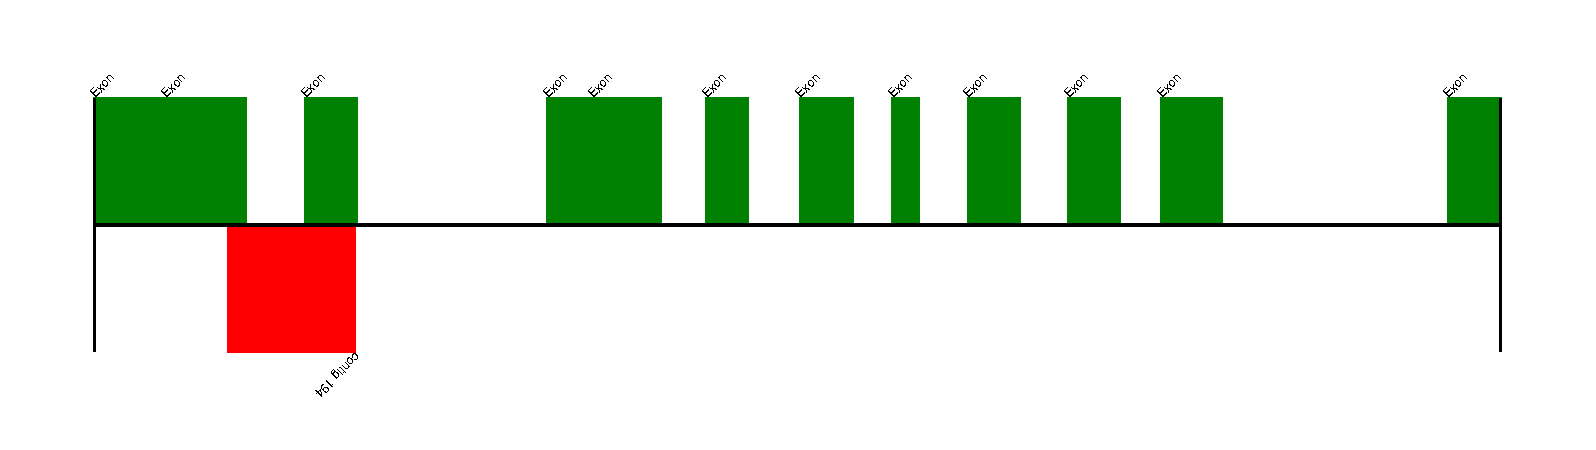
\includegraphics[width=\textwidth]{diag_genes/TRIUR3_14643.eps}
\end{minipage}

\begin{minipage}{\textwidth}
\centering{\bf{\large{Diagramme du gène TRIUR3\_14151}}}

\centering{Taille de la séquence: 5122 nucléotides}

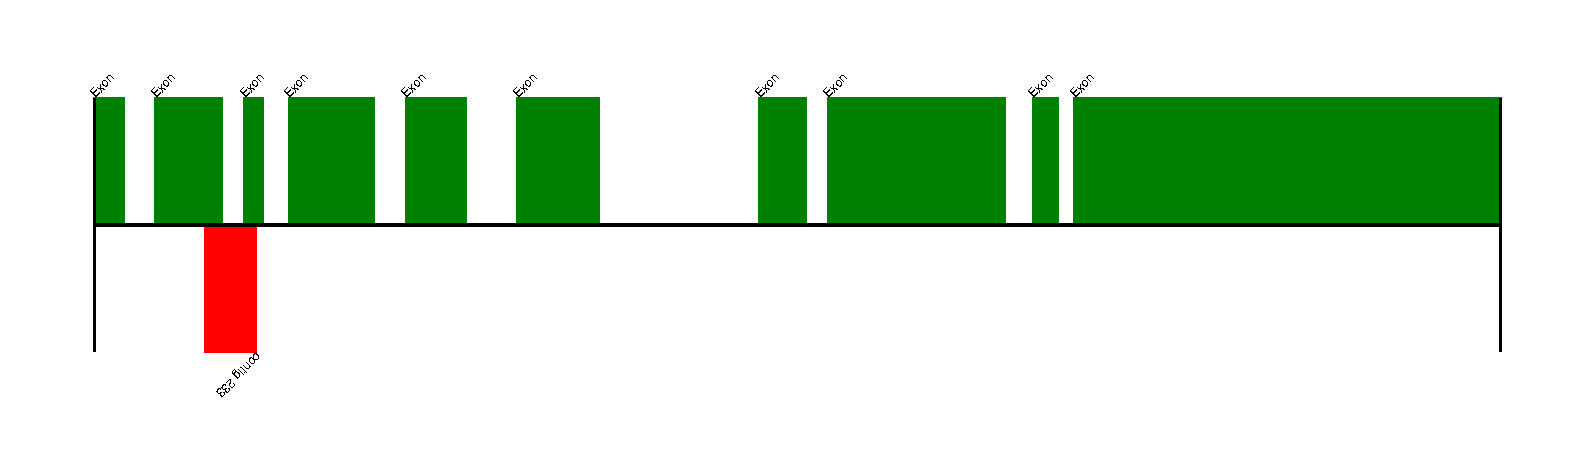
\includegraphics[width=\textwidth]{diag_genes/TRIUR3_14151.eps}
\end{minipage}

\begin{minipage}{\textwidth}
\centering{\bf{\large{Diagramme du gène TRIUR3\_13173}}}

\centering{Taille de la séquence: 756 nucléotides}


\includegraphics[width=\textwidth]{diag_genes/TRIUR3_13173.eps}
\end{minipage}

\begin{minipage}{\textwidth}
\centering{\bf{\large{Diagramme du gène TRIUR3\_02173}}}

\centering{Taille de la séquence: 153 nucléotides}


\includegraphics[width=\textwidth]{diag_genes/TRIUR3_02173.eps}
\end{minipage}

\begin{minipage}{\textwidth}
\centering{\bf{\large{Diagramme du gène TRIUR3\_00113}}}

\centering{Taille de la séquence: 279 nucléotides}


\includegraphics[width=\textwidth]{diag_genes/TRIUR3_00113.eps}
\end{minipage}

\begin{minipage}{\textwidth}
\centering{\bf{\large{Diagramme du gène TRIUR3\_30937}}}

\centering{Taille de la séquence: 2946 nucléotides}

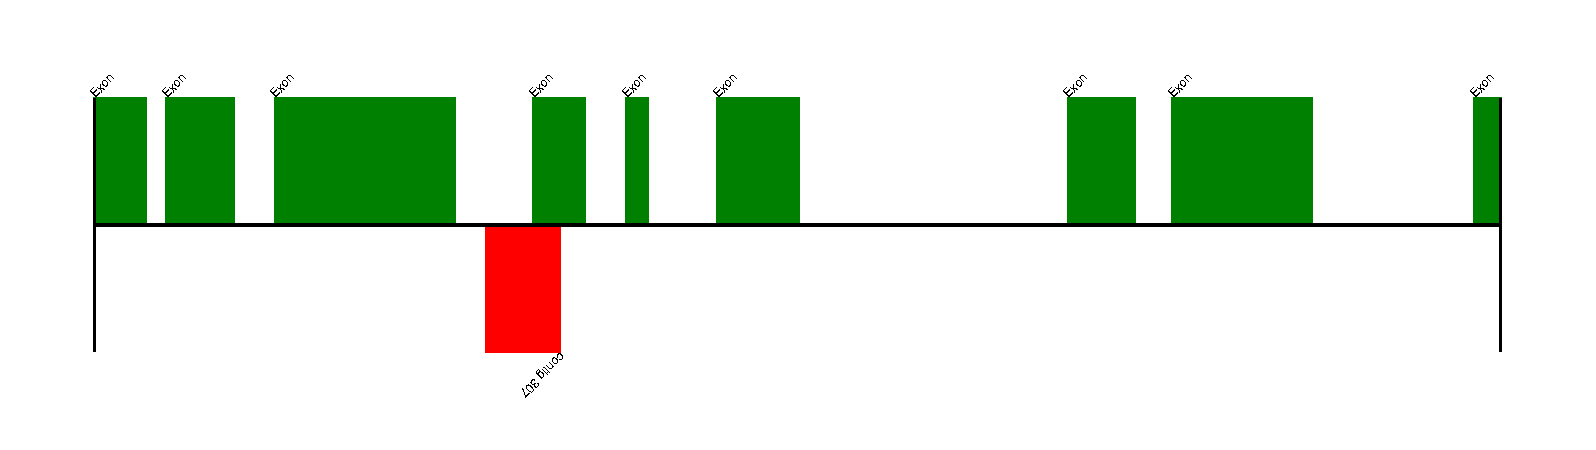
\includegraphics[width=\textwidth]{diag_genes/TRIUR3_30937.eps}
\end{minipage}

\begin{minipage}{\textwidth}
\centering{\bf{\large{Diagramme du gène TRIUR3\_27641}}}

\centering{Taille de la séquence: 5950 nucléotides}


\includegraphics[width=\textwidth]{diag_genes/TRIUR3_27641.eps}
\end{minipage}

\begin{minipage}{\textwidth}
\centering{\bf{\large{Diagramme du gène TRIUR3\_13694}}}

\centering{Taille de la séquence: 3585 nucléotides}

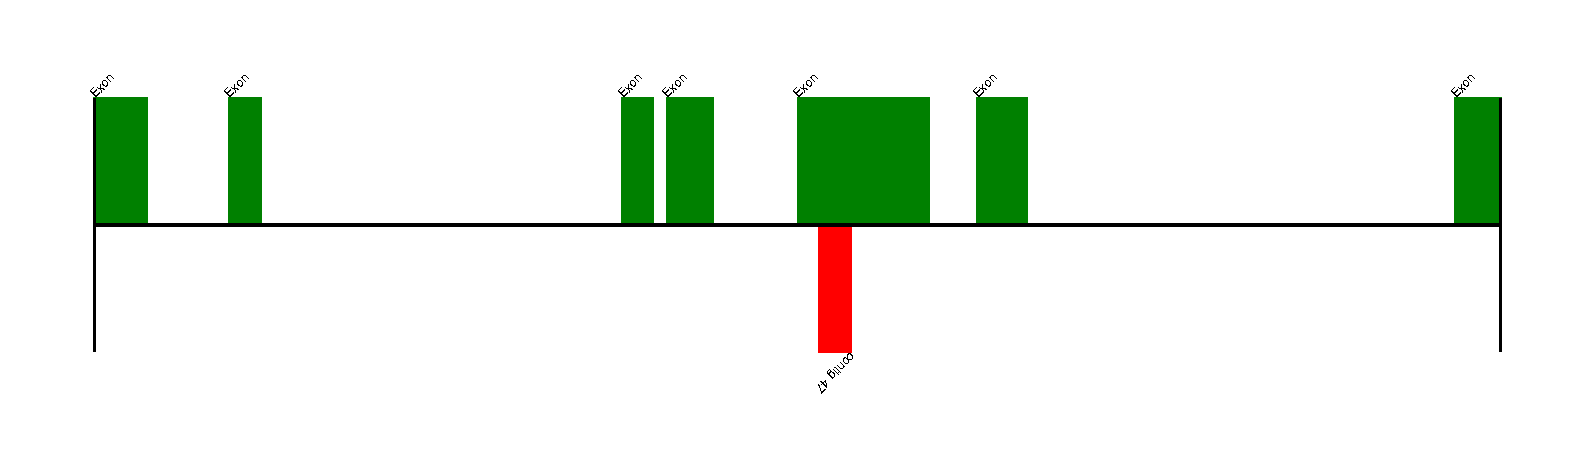
\includegraphics[width=\textwidth]{diag_genes/TRIUR3_13694.eps}
\end{minipage}

\begin{minipage}{\textwidth}
\centering{\bf{\large{Diagramme du gène TRIUR3\_10936}}}

\centering{Taille de la séquence: 5197 nucléotides}

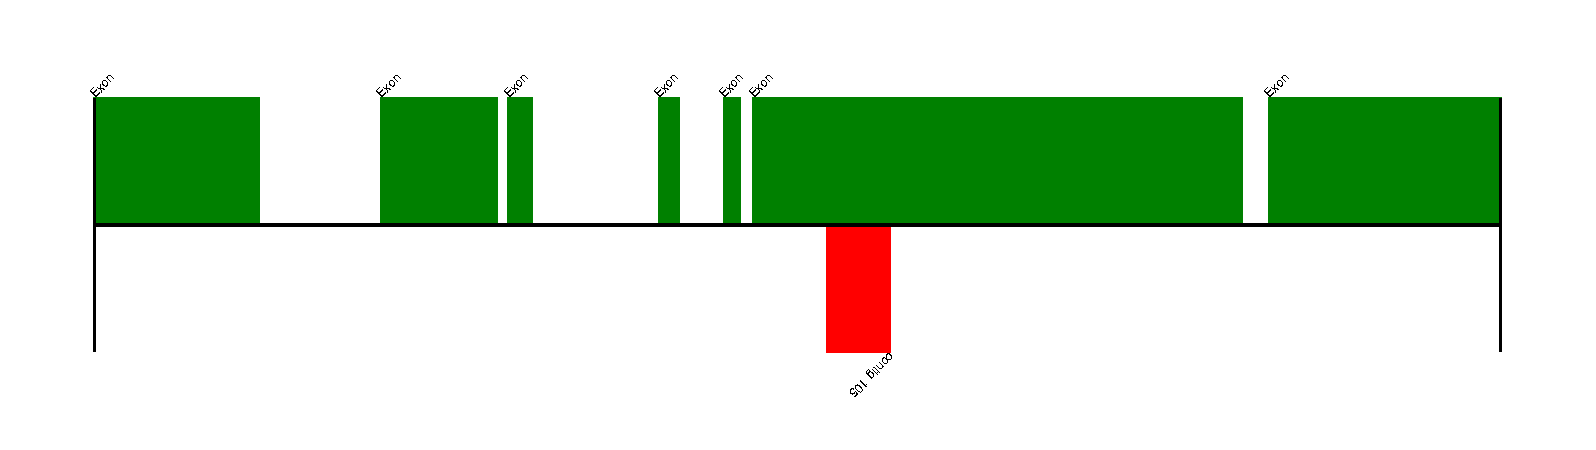
\includegraphics[width=\textwidth]{diag_genes/TRIUR3_10936.eps}
\end{minipage}

\begin{minipage}{\textwidth}
\centering{\bf{\large{Diagramme du gène TRIUR3\_27038}}}

\centering{Taille de la séquence: 5799 nucléotides}

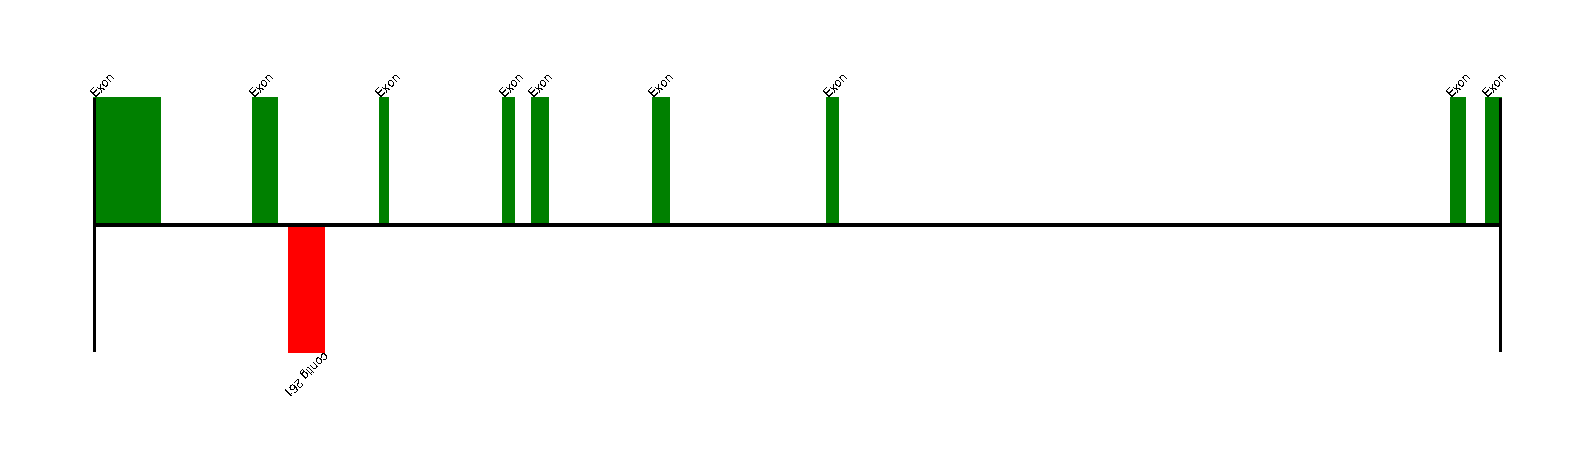
\includegraphics[width=\textwidth]{diag_genes/TRIUR3_27038.eps}
\end{minipage}

\begin{minipage}{\textwidth}
\centering{\bf{\large{Diagramme du gène TRIUR3\_34300}}}

\centering{Taille de la séquence: 747 nucléotides}


\includegraphics[width=\textwidth]{diag_genes/TRIUR3_34300.eps}
\end{minipage}

\begin{minipage}{\textwidth}
\centering{\bf{\large{Diagramme du gène TRIUR3\_23579}}}

\centering{Taille de la séquence: 4278 nucléotides}


\includegraphics[width=\textwidth]{diag_genes/TRIUR3_23579.eps}
\end{minipage}

\begin{minipage}{\textwidth}
\centering{\bf{\large{Diagramme du gène TRIUR3\_25715}}}

\centering{Taille de la séquence: 2599 nucléotides}

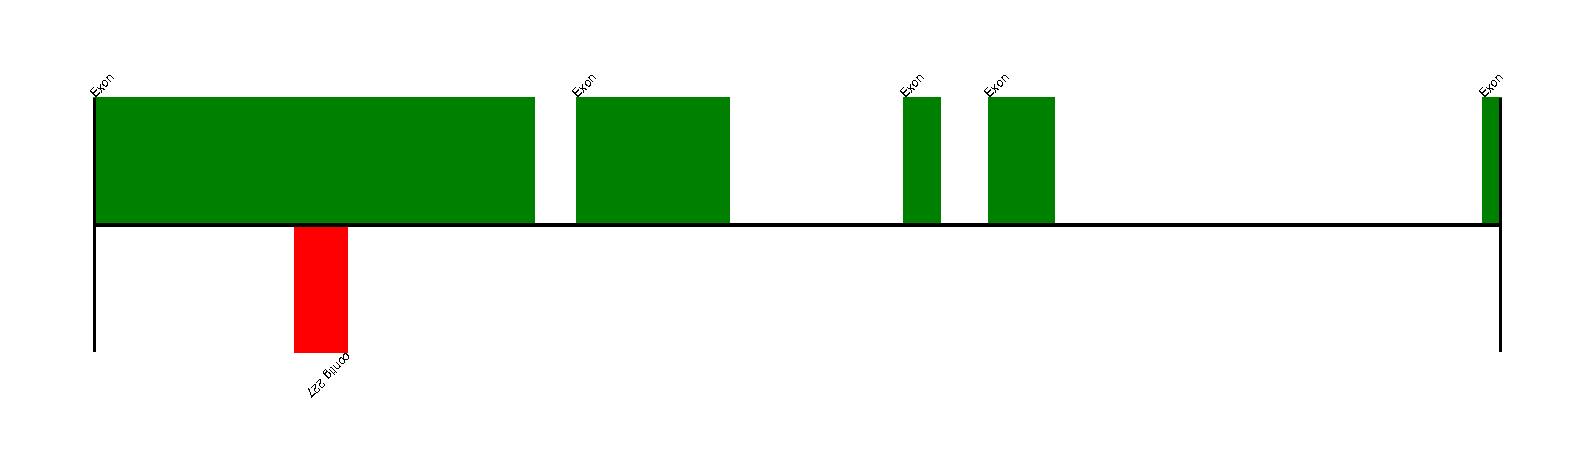
\includegraphics[width=\textwidth]{diag_genes/TRIUR3_25715.eps}
\end{minipage}

\begin{minipage}{\textwidth}
\centering{\bf{\large{Diagramme du gène TRIUR3\_26676}}}

\centering{Taille de la séquence: 3563 nucléotides}


\includegraphics[width=\textwidth]{diag_genes/TRIUR3_26676.eps}
\end{minipage}

\begin{minipage}{\textwidth}
\centering{\bf{\large{Diagramme du gène TRIUR3\_27314}}}

\centering{Taille de la séquence: 9511 nucléotides}

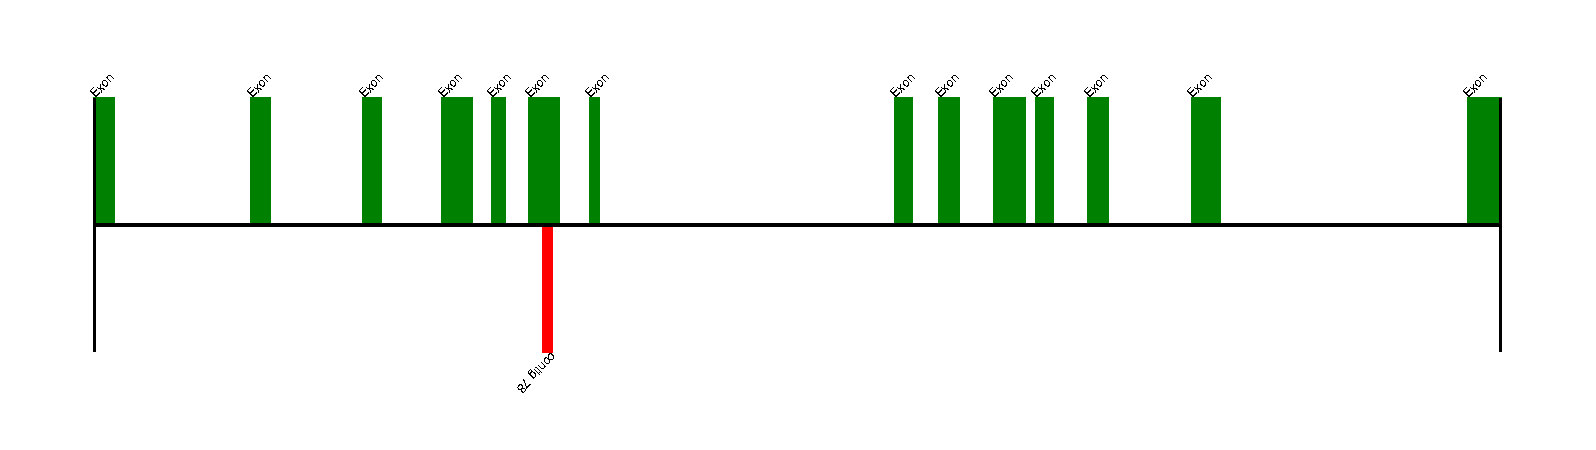
\includegraphics[width=\textwidth]{diag_genes/TRIUR3_27314.eps}
\end{minipage}

\begin{minipage}{\textwidth}
\centering{\bf{\large{Diagramme du gène TRIUR3\_02411}}}

\centering{Taille de la séquence: 6646 nucléotides}

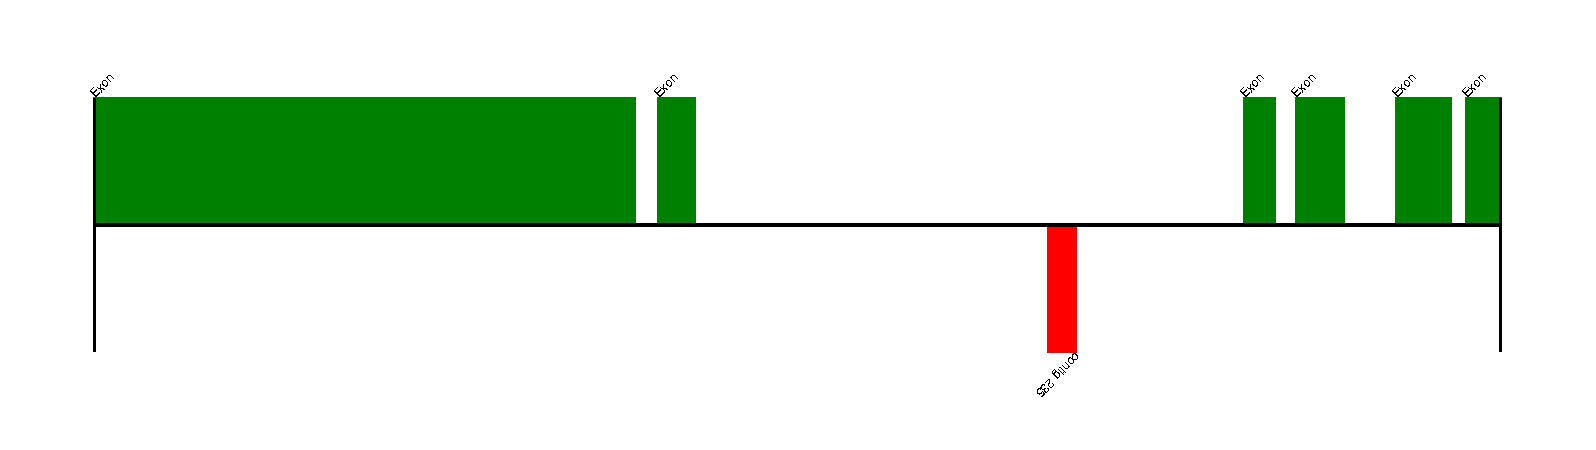
\includegraphics[width=\textwidth]{diag_genes/TRIUR3_02411.eps}
\end{minipage}

\begin{minipage}{\textwidth}
\centering{\bf{\large{Diagramme du gène TRIUR3\_03073}}}

\centering{Taille de la séquence: 4500 nucléotides}

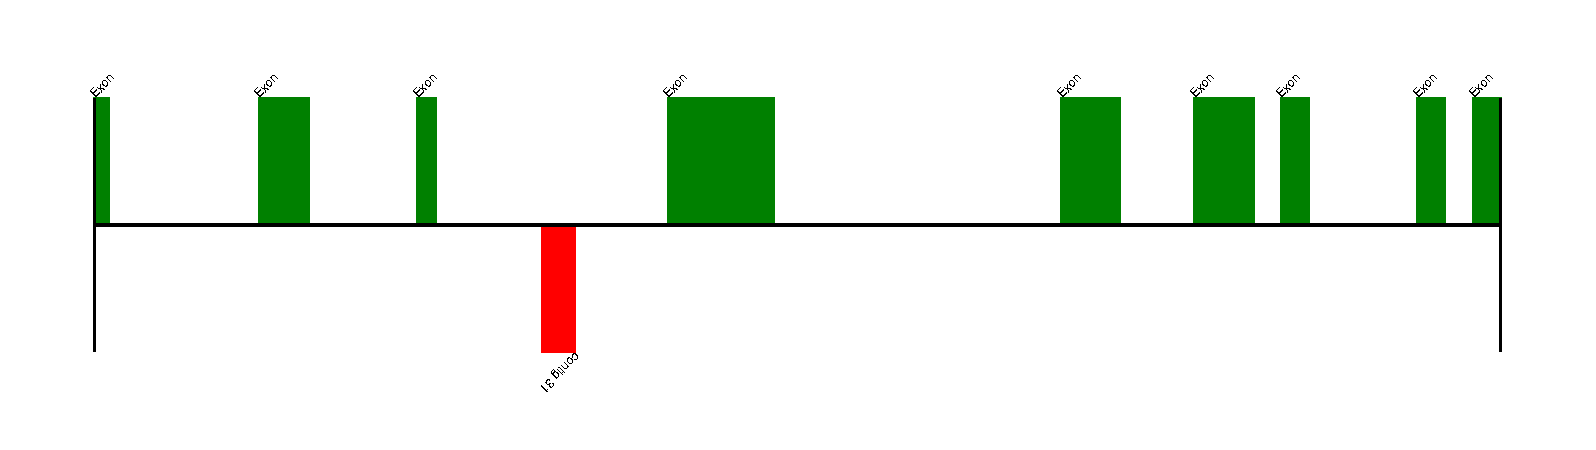
\includegraphics[width=\textwidth]{diag_genes/TRIUR3_03073.eps}
\end{minipage}

\begin{minipage}{\textwidth}
\centering{\bf{\large{Diagramme du gène TRIUR3\_07502}}}

\centering{Taille de la séquence: 3615 nucléotides}

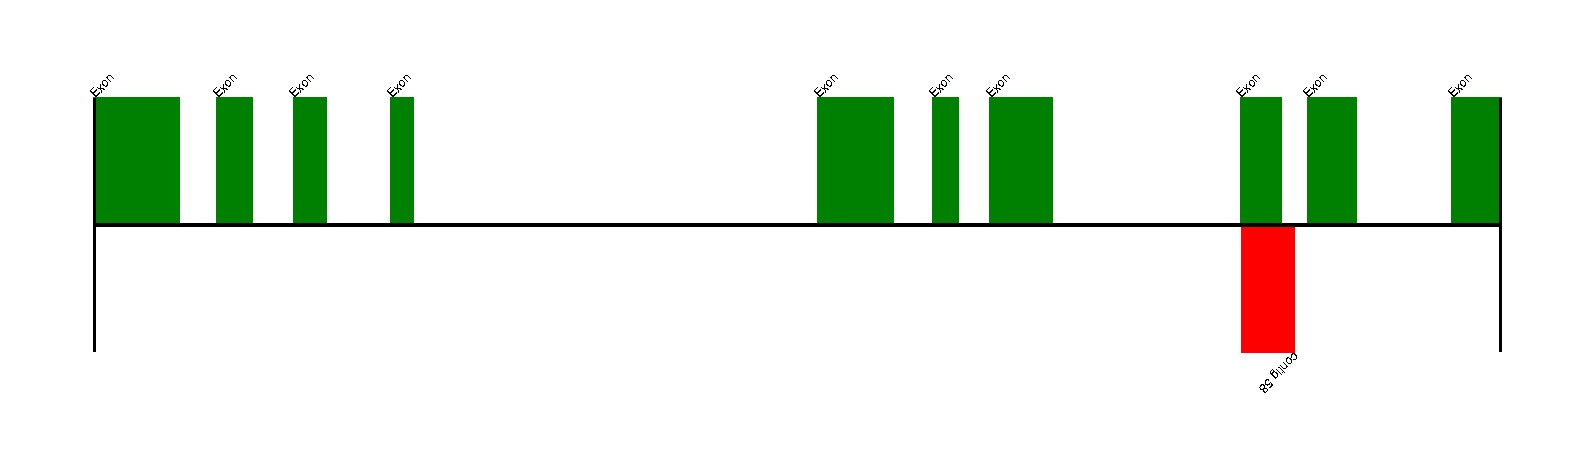
\includegraphics[width=\textwidth]{diag_genes/TRIUR3_07502.eps}
\end{minipage}

\begin{minipage}{\textwidth}
\centering{\bf{\large{Diagramme du gène TRIUR3\_13503}}}

\centering{Taille de la séquence: 4089 nucléotides}

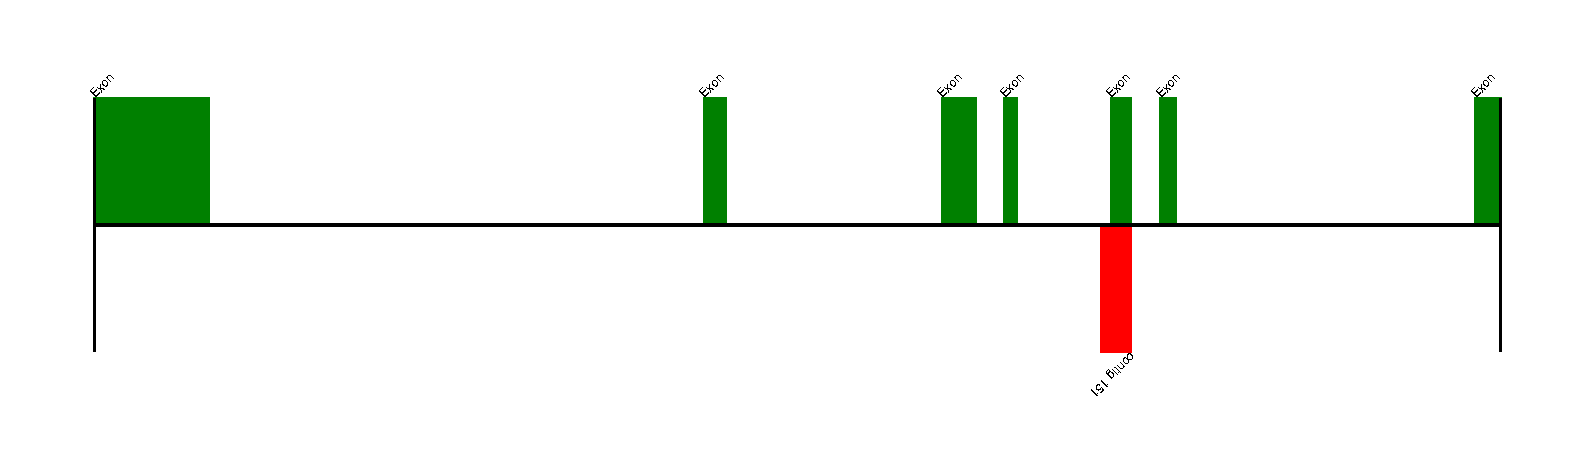
\includegraphics[width=\textwidth]{diag_genes/TRIUR3_13503.eps}
\end{minipage}

\begin{minipage}{\textwidth}
\centering{\bf{\large{Diagramme du gène TRIUR3\_07487}}}

\centering{Taille de la séquence: 4887 nucléotides}

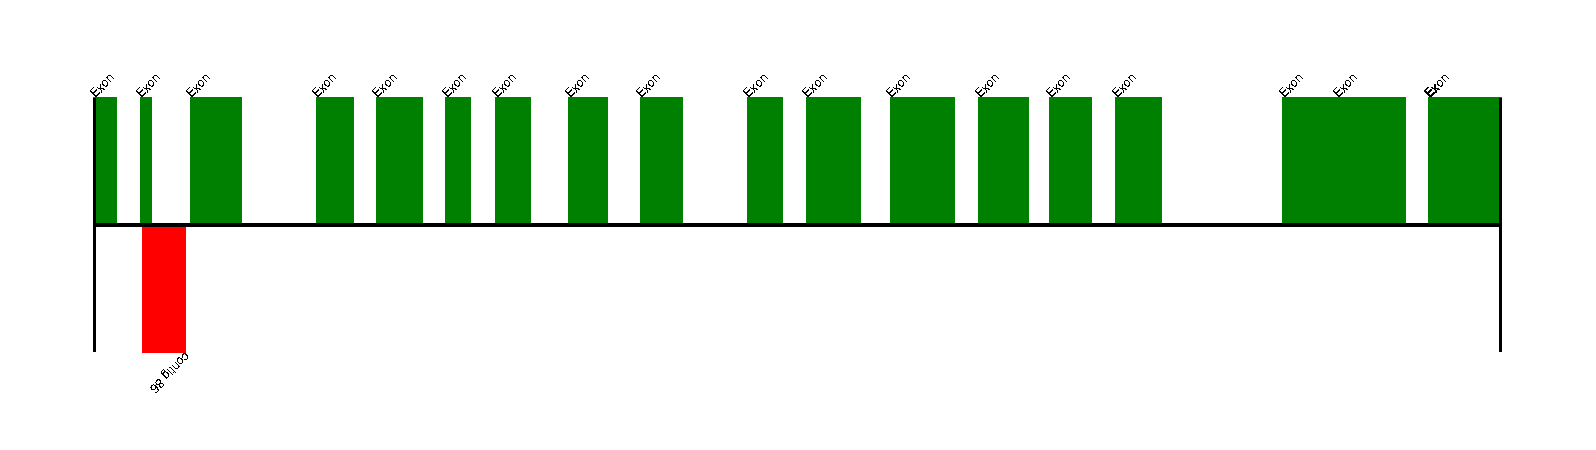
\includegraphics[width=\textwidth]{diag_genes/TRIUR3_07487.eps}
\end{minipage}

\begin{minipage}{\textwidth}
\centering{\bf{\large{Diagramme du gène TRIUR3\_05333}}}

\centering{Taille de la séquence: 1856 nucléotides}


\includegraphics[width=\textwidth]{diag_genes/TRIUR3_05333.eps}
\end{minipage}

\begin{minipage}{\textwidth}
\centering{\bf{\large{Diagramme du gène Phenylalanine ammonia-lyase (PAL)}}}

\centering{Taille de la séquence: 2924 nucléotides}


\includegraphics[width=\textwidth]{diag_genes/PAL.eps}
\end{minipage}

\begin{minipage}{\textwidth}
\centering{\bf{\large{Diagramme du gène TRIUR3\_27725}}}

\centering{Taille de la séquence: 1641 nucléotides}


\includegraphics[width=\textwidth]{diag_genes/TRIUR3_27725.eps}
\end{minipage}

\begin{minipage}{\textwidth}
\centering{\bf{\large{Diagramme du gène TRIUR3\_08705}}}

\centering{Taille de la séquence: 4719 nucléotides}


\includegraphics[width=\textwidth]{diag_genes/TRIUR3_08705.eps}
\end{minipage}

\begin{minipage}{\textwidth}
\centering{\bf{\large{Diagramme du gène TRIUR3\_33541}}}

\centering{Taille de la séquence: 3678 nucléotides}

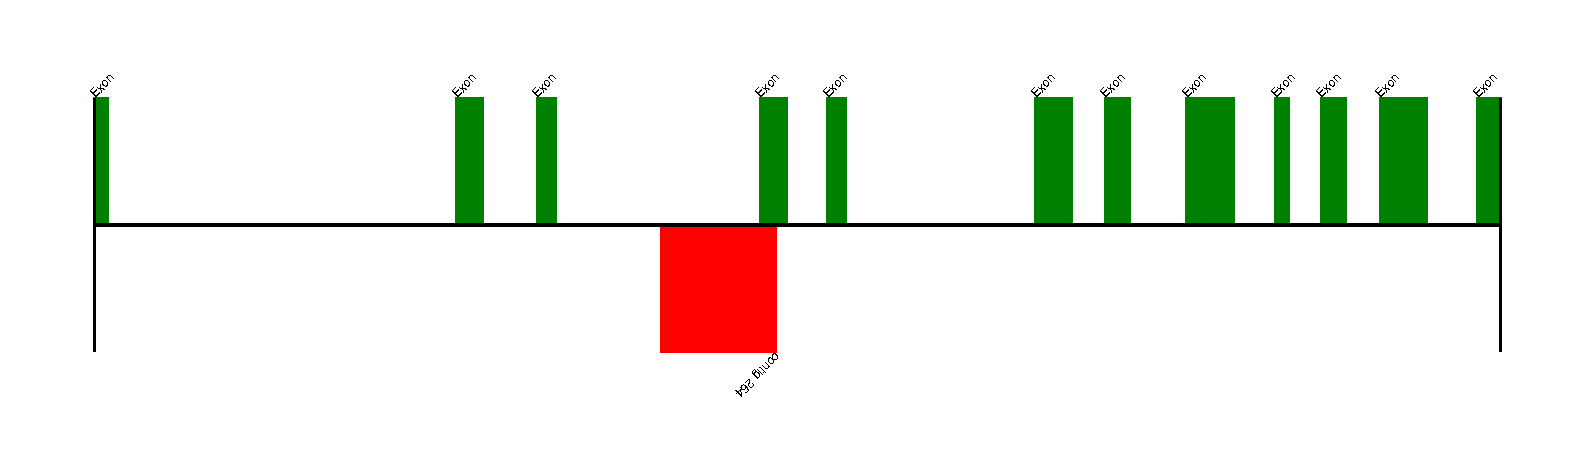
\includegraphics[width=\textwidth]{diag_genes/TRIUR3_33541.eps}
\end{minipage}

\begin{minipage}{\textwidth}
\centering{\bf{\large{Diagramme du gène TRIUR3\_33179}}}

\centering{Taille de la séquence: 14319 nucléotides}


\includegraphics[width=\textwidth]{diag_genes/TRIUR3_33179.eps}
\end{minipage}

\begin{minipage}{\textwidth}
\centering{\bf{\large{Diagramme du gène Glutamate dehydrogenase (Ta.5091)}}}


\includegraphics[width=\textwidth]{diag_genes/Ta_5091.eps}
\end{minipage}

\begin{minipage}{\textwidth}
\centering{\bf{\large{Diagramme du gène Triticum aestivum Unigene32879 (Ta.78700)}}}


\includegraphics[width=\textwidth]{diag_genes/Ta_78700.eps}
\end{minipage}

\begin{minipage}{\textwidth}
\centering{\bf{\large{Diagramme du gène TRIUR3\_05274}}}

\centering{Taille de la séquence: 3227 nucléotides}

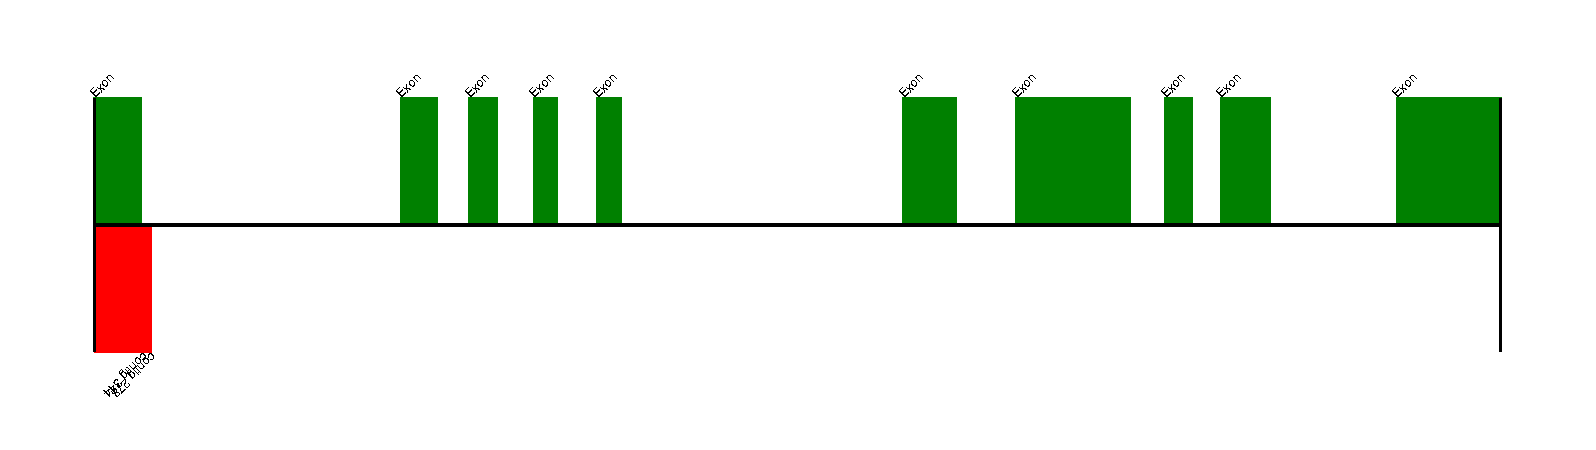
\includegraphics[width=\textwidth]{diag_genes/TRIUR3_05274.eps}
\end{minipage}

\begin{minipage}{\textwidth}
\centering{\bf{\large{Diagramme du gène Mla-like protein (AY487917)}}}


\includegraphics[width=\textwidth]{diag_genes/AY487917.eps}
\end{minipage}

\begin{minipage}{\textwidth}
\centering{\bf{\large{Diagramme du gène Gliadin/avenin-like seed protein (Ta.2415)}}}


\includegraphics[width=\textwidth]{diag_genes/Ta_2415.eps}
\end{minipage}

\begin{minipage}{\textwidth}
\centering{\bf{\large{Diagramme du gène TRIUR3\_19685}}}

\centering{Taille de la séquence: 12586 nucléotides}


\includegraphics[width=\textwidth]{diag_genes/TRIUR3_19685.eps}
\end{minipage}

\begin{minipage}{\textwidth}
\centering{\bf{\large{Diagramme du gène TRIUR3\_01363}}}

\centering{Taille de la séquence: 2191 nucléotides}


\includegraphics[width=\textwidth]{diag_genes/TRIUR3_01363.eps}
\end{minipage}

\begin{minipage}{\textwidth}
\centering{\bf{\large{Diagramme du gène TRIUR3\_12227}}}

\centering{Taille de la séquence: 2142 nucléotides}


\includegraphics[width=\textwidth]{diag_genes/TRIUR3_12227.eps}
\end{minipage}

\begin{minipage}{\textwidth}
\centering{\bf{\large{Diagramme du gène TRIUR3\_22350}}}

\centering{Taille de la séquence: 8138 nucléotides}

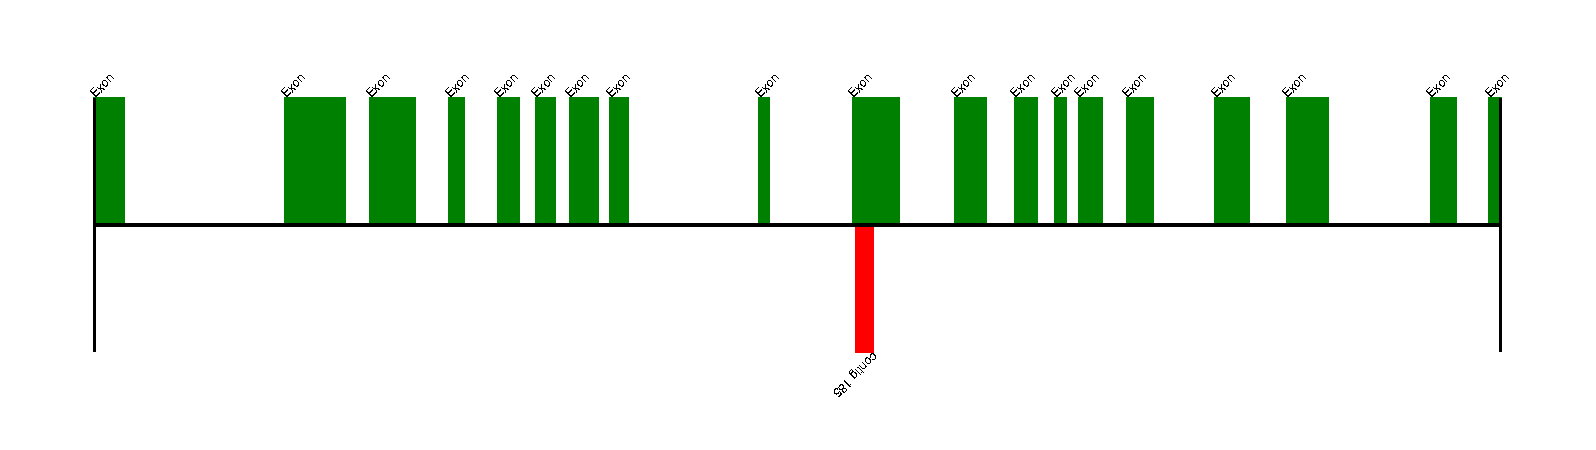
\includegraphics[width=\textwidth]{diag_genes/TRIUR3_22350.eps}
\end{minipage}

\begin{minipage}{\textwidth}
\centering{\bf{\large{Diagramme du gène TRIUR3\_16229}}}

\centering{Taille de la séquence: 321 nucléotides}


\includegraphics[width=\textwidth]{diag_genes/TRIUR3_16229.eps}
\end{minipage}

\begin{minipage}{\textwidth}
\centering{\bf{\large{Diagramme du gène TRIUR3\_14429}}}

\centering{Taille de la séquence: 4058 nucléotides}

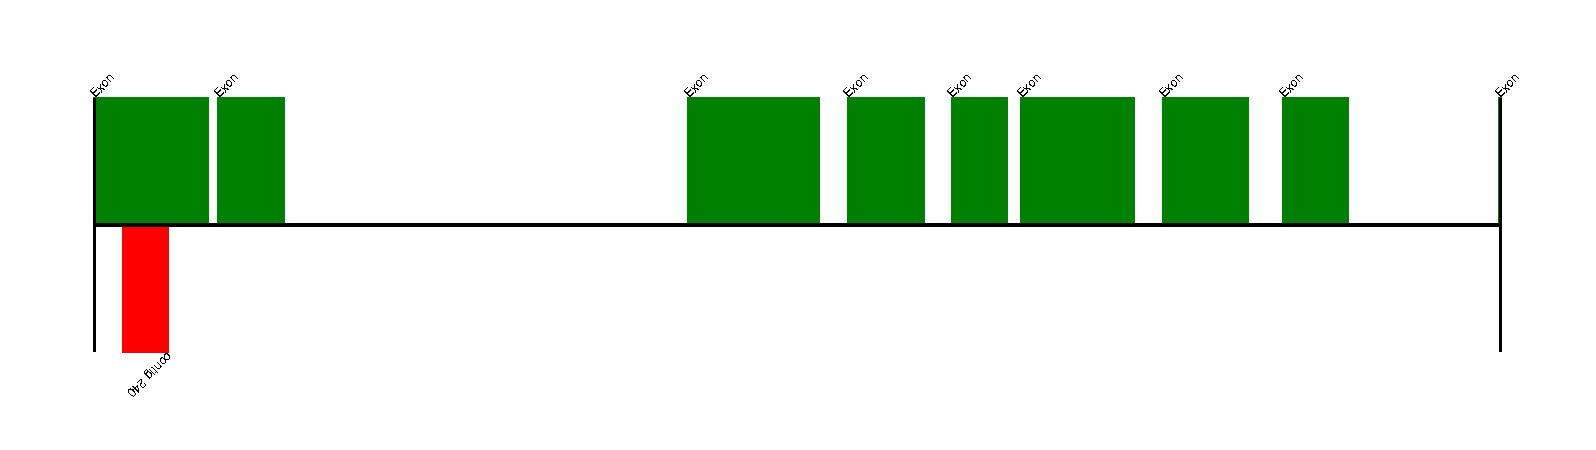
\includegraphics[width=\textwidth]{diag_genes/TRIUR3_14429.eps}
\end{minipage}

\begin{minipage}{\textwidth}
\centering{\bf{\large{Diagramme du gène TRIUR3\_20221}}}

\centering{Taille de la séquence: 4115 nucléotides}

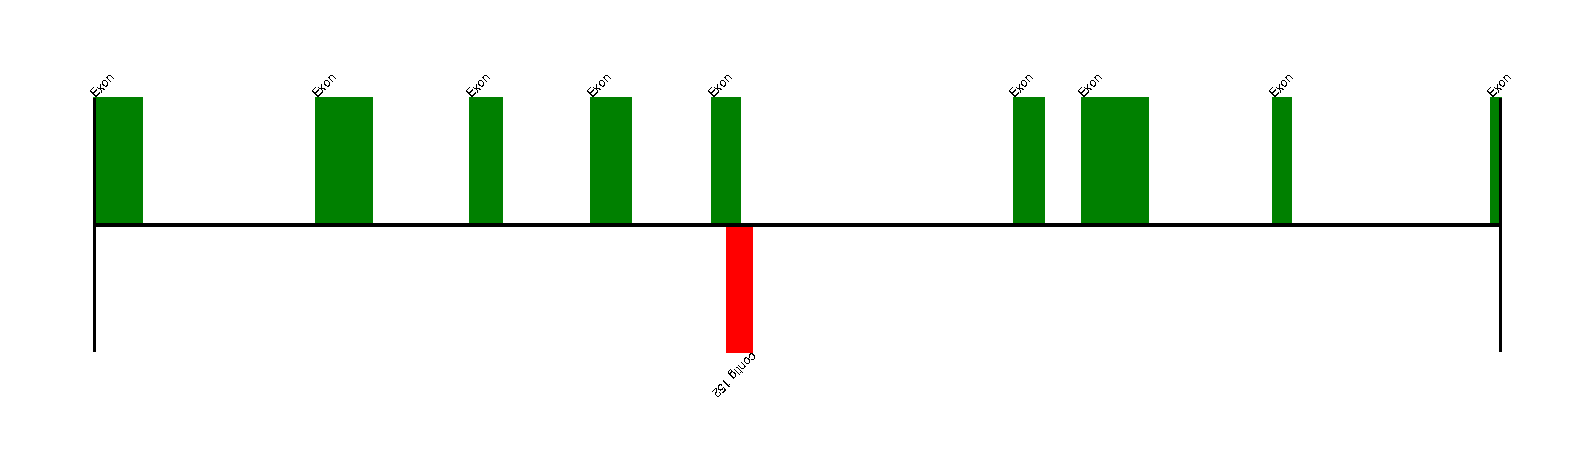
\includegraphics[width=\textwidth]{diag_genes/TRIUR3_20221.eps}
\end{minipage}

\begin{minipage}{\textwidth}
\centering{\bf{\large{Diagramme du gène TRIUR3\_13835}}}

\centering{Taille de la séquence: 5947 nucléotides}

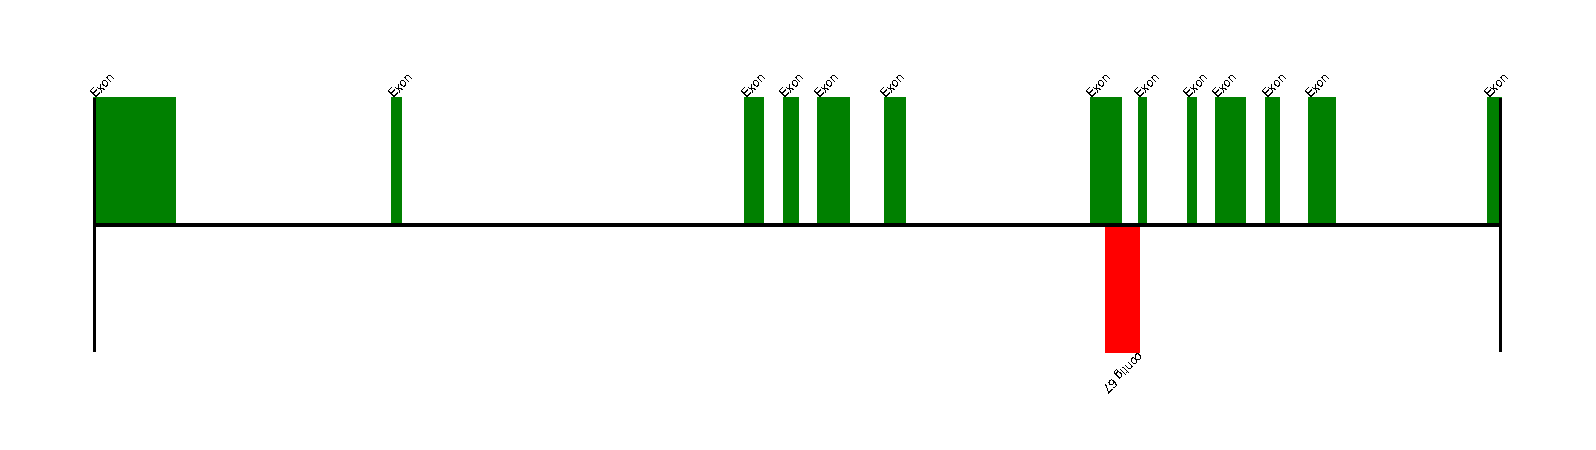
\includegraphics[width=\textwidth]{diag_genes/TRIUR3_13835.eps}
\end{minipage}

\begin{minipage}{\textwidth}
\centering{\bf{\large{Diagramme du gène TRIUR3\_05438}}}

\centering{Taille de la séquence: 663 nucléotides}

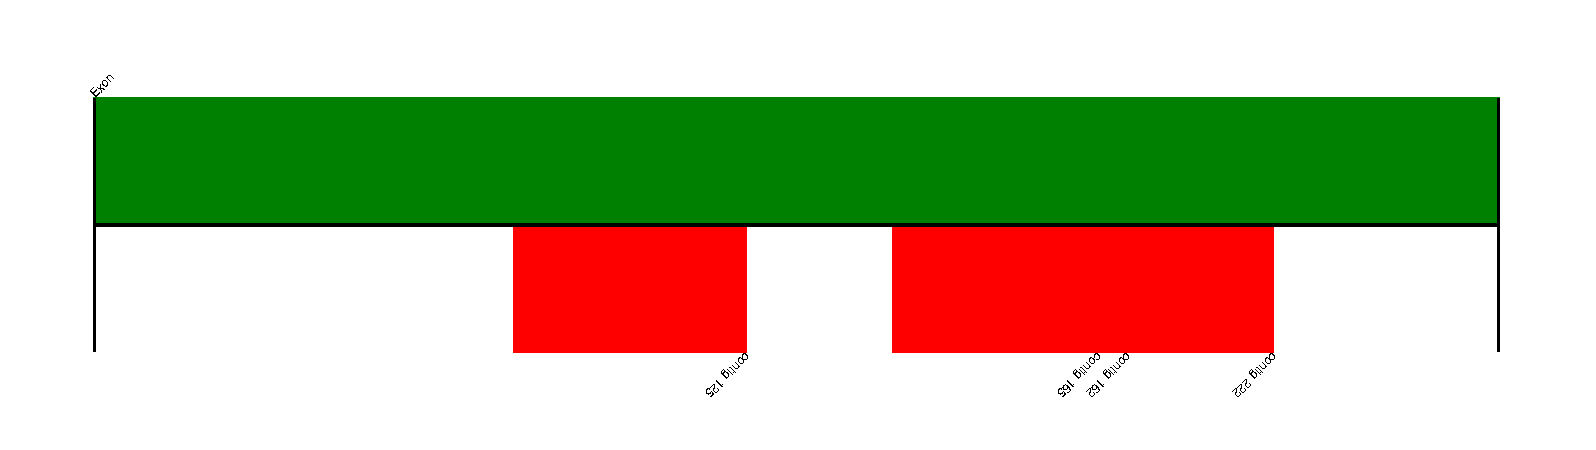
\includegraphics[width=\textwidth]{diag_genes/TRIUR3_05438.eps}
\end{minipage}

\begin{minipage}{\textwidth}
\centering{\bf{\large{Diagramme du gène TRIUR3\_30579}}}

\centering{Taille de la séquence: 16467 nucléotides}

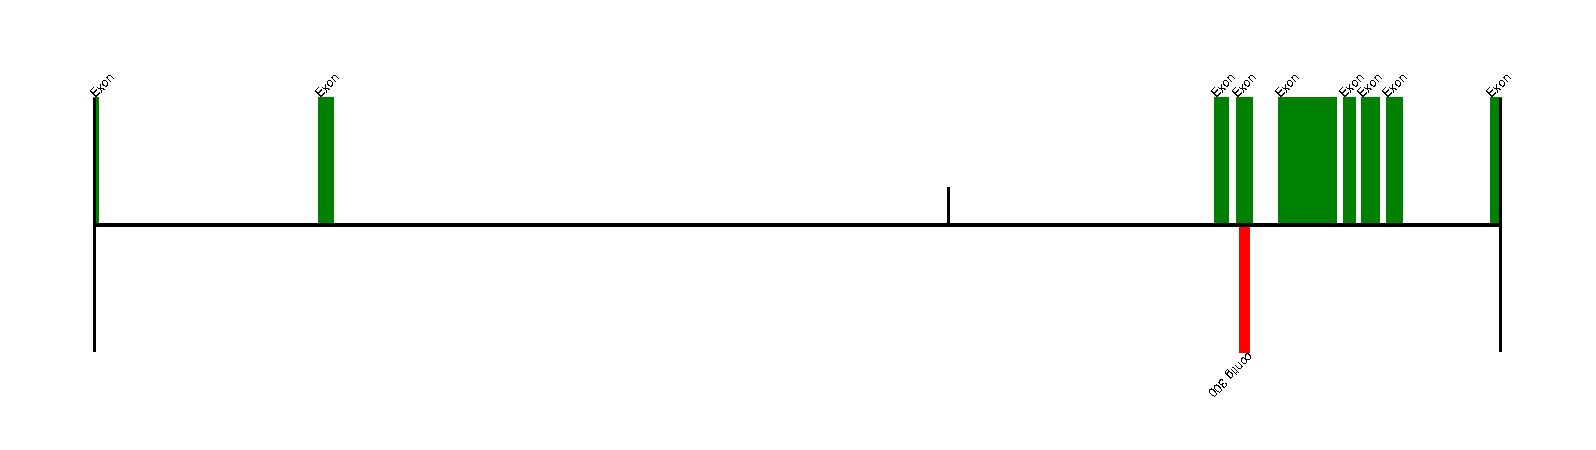
\includegraphics[width=\textwidth]{diag_genes/TRIUR3_30579.eps}
\end{minipage}

\begin{minipage}{\textwidth}
\centering{\bf{\large{Diagramme du gène TRIUR3\_23654}}}

\centering{Taille de la séquence: 4219 nucléotides}

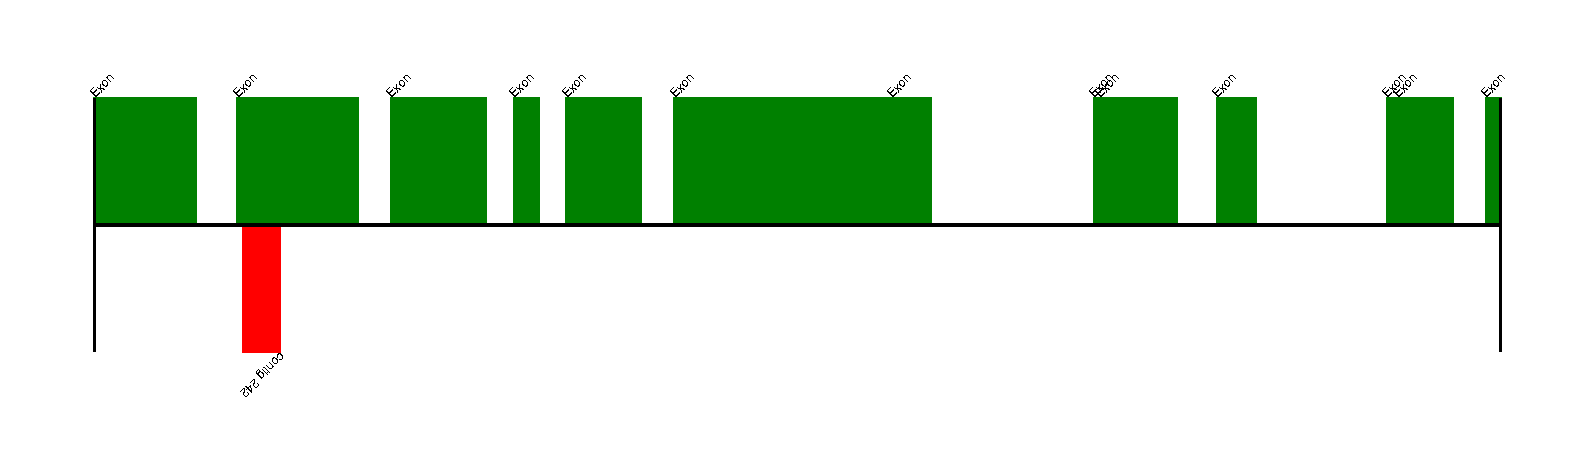
\includegraphics[width=\textwidth]{diag_genes/TRIUR3_23654.eps}
\end{minipage}

\begin{minipage}{\textwidth}
\centering{\bf{\large{Diagramme du gène TRIUR3\_23427}}}

\centering{Taille de la séquence: 4426 nucléotides}

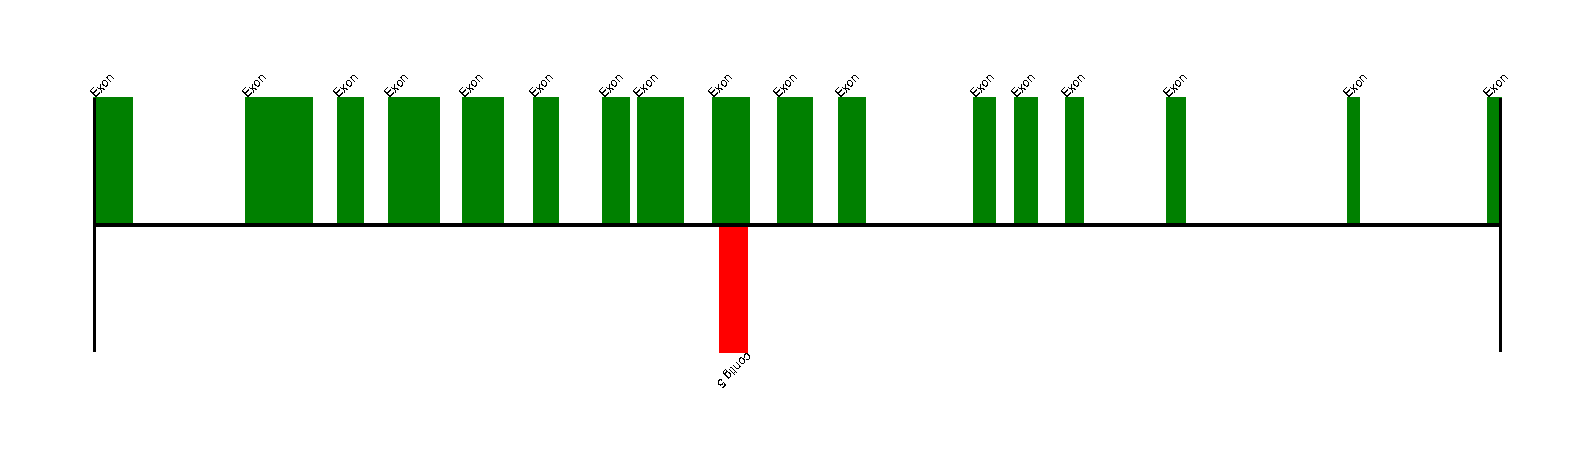
\includegraphics[width=\textwidth]{diag_genes/TRIUR3_23427.eps}
\end{minipage}

\begin{minipage}{\textwidth}
\centering{\bf{\large{Diagramme du gène TRIUR3\_18045}}}

\centering{Taille de la séquence: 3789 nucléotides}

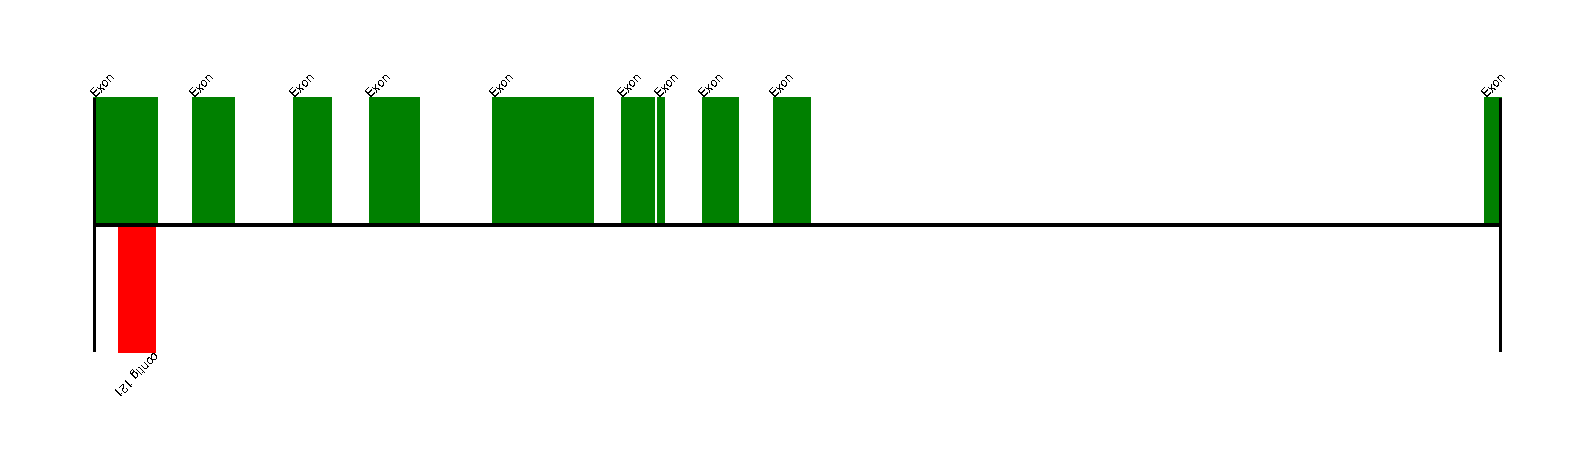
\includegraphics[width=\textwidth]{diag_genes/TRIUR3_18045.eps}
\end{minipage}

\begin{minipage}{\textwidth}
\centering{\bf{\large{Diagramme du gène TRIUR3\_12384}}}

\centering{Taille de la séquence: 1750 nucléotides}

\includegraphics[width=\textwidth]{diag_genes/TRIUR3_12384.eps}
\end{minipage}

\begin{minipage}{\textwidth}
\centering{\bf{\large{Diagramme du gène TRIUR3\_28576}}}

\centering{Taille de la séquence: 7184 nucléotides}

\includegraphics[width=\textwidth]{diag_genes/TRIUR3_28576.eps}
\end{minipage}

\begin{minipage}{\textwidth}
\centering{\bf{\large{Diagramme du gène TRIUR3\_31408}}}

\centering{Taille de la séquence: 4209 nucléotides}

\includegraphics[width=\textwidth]{diag_genes/TRIUR3_31408.eps}
\end{minipage}

\begin{minipage}{\textwidth}
\centering{\bf{\large{Diagramme du gène Voltage dependent anion channel (VDAC) (TAVDAC3)}}}

\centering{Taille de la séquence: 2461 nucléotides}

\includegraphics[width=\textwidth]{diag_genes/TAVDAC3.eps}
\end{minipage}

\begin{minipage}{\textwidth}
\centering{\bf{\large{Diagramme du gène TRIUR3\_03695}}}

\centering{Taille de la séquence: 2516 nucléotides}

\includegraphics[width=\textwidth]{diag_genes/TRIUR3_03695.eps}
\end{minipage}

\begin{minipage}{\textwidth}
\centering{\bf{\large{Diagramme du gène TRIUR3\_07580}}}

\centering{Taille de la séquence: 4786 nucléotides}

\includegraphics[width=\textwidth]{diag_genes/TRIUR3_07580.eps}
\end{minipage}

\begin{minipage}{\textwidth}
\centering{\bf{\large{Diagramme du gène Sucrose phosphate synthase II (GU797179)}}}

\includegraphics[width=\textwidth]{diag_genes/GU797179.eps}
\end{minipage}

\begin{minipage}{\textwidth}
\centering{\bf{\large{Diagramme du gène TRIUR3\_29691}}}

\centering{Taille de la séquence: 1892 nucléotides}

\includegraphics[width=\textwidth]{diag_genes/TRIUR3_29691.eps}
\end{minipage}

\begin{minipage}{\textwidth}
\centering{\bf{\large{Diagramme du gène TRIUR3\_14115}}}

\centering{Taille de la séquence: 2485 nucléotides}

\includegraphics[width=\textwidth]{diag_genes/TRIUR3_14115.eps}
\end{minipage}

\begin{minipage}{\textwidth}
\centering{\bf{\large{Diagramme du gène TRIUR3\_07936}}}

\centering{Taille de la séquence: 3813 nucléotides}

\includegraphics[width=\textwidth]{diag_genes/TRIUR3_07936.eps}
\end{minipage}

\begin{minipage}{\textwidth}
\centering{\bf{\large{Diagramme du gène TRIUR3\_10330}}}

\centering{Taille de la séquence: 3728 nucléotides}

\includegraphics[width=\textwidth]{diag_genes/TRIUR3_10330.eps}
\end{minipage}

\begin{minipage}{\textwidth}
\centering{\bf{\large{Diagramme du gène TRIUR3\_19087}}}

\centering{Taille de la séquence: 4533 nucléotides}

\includegraphics[width=\textwidth]{diag_genes/TRIUR3_19087.eps}
\end{minipage}

\begin{minipage}{\textwidth}
\centering{\bf{\large{Diagramme du gène Replication factor C subunit 1 (RFC-1)}}}

\includegraphics[width=\textwidth]{diag_genes/RFC-1.eps}
\end{minipage}

\begin{minipage}{\textwidth}
\centering{\bf{\large{Diagramme du gène TRIUR3\_27124}}}

\centering{Taille de la séquence: 6393 nucléotides}

\includegraphics[width=\textwidth]{diag_genes/TRIUR3_27124.eps}
\end{minipage}

\begin{minipage}{\textwidth}
\centering{\bf{\large{Diagramme du gène TRIUR3\_30764}}}

\centering{Taille de la séquence: 22944 nucléotides}

\includegraphics[width=\textwidth]{diag_genes/TRIUR3_30764.eps}
\end{minipage}

\begin{minipage}{\textwidth}
\centering{\bf{\large{Diagramme du gène TRIUR3\_05640}}}

\centering{Taille de la séquence: 4604 nucléotides}

\includegraphics[width=\textwidth]{diag_genes/TRIUR3_05640.eps}
\end{minipage}

\begin{minipage}{\textwidth}
\centering{\bf{\large{Diagramme du gène SNF1-related protein kinase (snRK1)}}}

\centering{Taille de la séquence: 4620 nucléotides}

\includegraphics[width=\textwidth]{diag_genes/snRK1.eps}
\end{minipage}

\begin{minipage}{\textwidth}
\centering{\bf{\large{Diagramme du gène TRIUR3\_00007}}}

\centering{Taille de la séquence: 303 nucléotides}

\includegraphics[width=\textwidth]{diag_genes/TRIUR3_00007.eps}
\end{minipage}

\begin{minipage}{\textwidth}
\centering{\bf{\large{Diagramme du gène TRIUR3\_11137}}}

\centering{Taille de la séquence: 3873 nucléotides}

\includegraphics[width=\textwidth]{diag_genes/TRIUR3_11137.eps}
\end{minipage}

\begin{minipage}{\textwidth}
\centering{\bf{\large{Diagramme du gène TRIUR3\_05845}}}

\centering{Taille de la séquence: 417 nucléotides}

\includegraphics[width=\textwidth]{diag_genes/TRIUR3_05845.eps}
\end{minipage}



\section{Conclusion}

Le but donné de ce travail était d'annoter et de cartographier des contigs provenant des ESTs du blé. J'ai choisi d'orienter
ma recherche directement dans les séquences, protéines et gènes déjà connus du blé. Donc, pour j'ai seulement recherché à annoter
les contigs pour lesquels j'avais des résultats de bonne qualité pour les résultats. J'ai défini cet élément de qualité par la
E-value du blast qui tentait d'associer le contig à une séquence connue. 

En vérifiant la E-value médiane des résultats selon la longueur du contig, j'ai remarqué que, malgré une différence dans l'ordre
de grandeur des E-value, les résultats pour les contigs plus courts étaient quand même de bonne qualité. J'ai donc appliqué la même
règle pour chaque contig.

Lorsque j'ai identifié si au moins un des résultats de blast était le blé, je n'ai pas tenu compte du nombre de hit correspondant
au blé. C'est une information qui aurait été intéressante à avoir, il aurait peut-être été possible de regrouper certains contigs
en un gène plutôt que d'avoir des gènes différents. Toutefois, comme les résultats du blast sur la base de données ont démontré, 
la plupart des contigs faisaient partie de différentes familles, ou clusters, de protéines, il est donc peu probable qu'il ait été
possible de les regrouper d'avantage.

Une analyse sommaire des résultats obtenus semblent indiquer que plusieurs des ESTS proviennent du chromosome 3 du blé. D'abord, car
les résultats des blasts ont trouvé un nombre de hits pour le chromosome 3B, mais aussi car les gènes identifiés proviennent en grande
partie du chromosome 3 du \emph{Triticum urartu}, une espèce utilisée pour tenter de prédire les gènes du blé.

Toutefois, je n'ai pas su comment mettre en place une façon de vérifier les résutlats obtenus. En effet, pour le moment, je vérifie
seulement la qualité du résultat si elle est donnée, par exemple, dans un blast, mais je n'ai aucune autre façon de vérifier si
j'obtiens bien le bon résultat.

Ce travail d'annotation et de cartographie représente une première étape à propos de l'identification de ces ESTs. IL aurait été 
possible d'étendre la recherche à des espèces proches du blé, qui sont mieux annotées présentement. Par exemple, le riz.

\begingroup
\renewcommand{\appendix}{%
    \renewcommand{\thesubsection}{\arabic{subsection}}
}

\newpage
\appendix
\section{Annexes}

\subsection{Tableau de la taille et du taux de GC des contigs}\label{1}

\footnotesize{
\begin{longtable}{|p{2cm}|p{2cm}|p{2cm}|p{2cm}|p{2cm}|p{2cm}|}
\hline
Contig & Taille & Taux GC & Contig & Taille & Taux GC\\
\hline
1 & 91& 51.65 & 2 & 182& 31.87\\
\hline
3 & 183& 42.62 & 4 & 103& 39.81\\
\hline
5 & 83& 42.17 & 6 & 90& 42.22\\
\hline
7 & 100& 46.00 & 8 & 88& 38.64\\
\hline
9 & 122& 33.61 & 10 & 110& 37.27\\
\hline
11 & 140& 43.57 & 12 & 96& 37.50\\
\hline
13 & 120& 37.50 & 14 & 114& 39.47\\
\hline
15 & 79& 64.56 & 16 & 238& 41.60\\
\hline
17 & 143& 55.24 & 18 & 97& 51.55\\
\hline
19 & 143& 53.85 & 20 & 82& 45.12\\
\hline
21 & 209& 45.45 & 22 & 105& 38.10\\
\hline
23 & 150& 48.67 & 24 & 102& 47.06\\
\hline
25 & 101& 36.63 & 26 & 88& 43.18\\
\hline
27 & 151& 35.76 & 28 & 137& 59.85\\
\hline
29 & 97& 44.33 & 30 & 112& 25.89\\
\hline
31 & 70& 38.57 & 32 & 125& 44.80\\
\hline
33 & 83& 40.96 & 34 & 95& 32.63\\
\hline
35 & 201& 38.31 & 36 & 203& 30.05\\
\hline
37 & 69& 79.71 & 38 & 153& 36.60\\
\hline
39 & 75& 44.00 & 40 & 96& 46.88\\
\hline
41 & 52& 44.23 & 42 & 74& 45.95\\
\hline
43 & 96& 63.54 & 44 & 115& 43.48\\
\hline
45 & 87& 44.83 & 46 & 96& 48.96\\
\hline
47 & 82& 45.12 & 48 & 125& 40.00\\
\hline
49 & 131& 35.88 & 50 & 102& 49.02\\
\hline
51 & 70& 47.14 & 52 & 80& 43.75\\
\hline
53 & 99& 42.42 & 54 & 124& 40.32\\
\hline
55 & 108& 45.37 & 56 & 142& 40.85\\
\hline
57 & 87& 36.78 & 58 & 133& 40.60\\
\hline
59 & 112& 33.04 & 60 & 90& 40.00\\
\hline
61 & 94& 44.68 & 62 & 95& 44.21\\
\hline
63 & 103& 44.66 & 64 & 185& 59.46\\
\hline
65 & 142& 41.55 & 66 & 99& 40.40\\
\hline
67 & 150& 49.33 & 68 & 84& 34.52\\
\hline
69 & 46& 50.00 & 70 & 110& 34.55\\
\hline
71 & 80& 47.50 & 72 & 134& 50.00\\
\hline
73 & 113& 53.10 & 74 & 93& 45.16\\
\hline
75 & 179& 36.87 & 76 & 82& 46.34\\
\hline
77 & 106& 42.45 & 78 & 61& 45.90\\
\hline
79 & 157& 31.21 & 80 & 111& 69.37\\
\hline
81 & 92& 47.83 & 82 & 183& 45.90\\
\hline
83 & 51& 39.22 & 84 & 143& 34.97\\
\hline
85 & 87& 40.23 & 86 & 102& 62.75\\
\hline
87 & 51& 29.41 & 88 & 116& 46.55\\
\hline
89 & 107& 42.99 & 90 & 76& 46.05\\
\hline
91 & 73& 47.95 & 92 & 104& 36.54\\
\hline
93 & 201& 45.27 & 94 & 85& 31.76\\
\hline
95 & 99& 41.41 & 96 & 108& 38.89\\
\hline
97 & 63& 33.33 & 98 & 131& 45.80\\
\hline
99 & 62& 25.81 & 100 & 111& 40.54\\
\hline
101 & 121& 38.84 & 102 & 109& 43.12\\
\hline
103 & 70& 37.14 & 104 & 148& 43.92\\
\hline
105 & 105& 46.67 & 106 & 103& 70.87\\
\hline
107 & 105& 37.14 & 108 & 104& 42.31\\
\hline
109 & 92& 41.30 & 110 & 80& 38.75\\
\hline
111 & 120& 22.50 & 112 & 101& 47.52\\
\hline
113 & 69& 44.93 & 114 & 76& 38.16\\
\hline
115 & 92& 76.09 & 116 & 69& 36.23\\
\hline
117 & 94& 47.87 & 118 & 55& 34.55\\
\hline
119 & 138& 67.39 & 120 & 112& 38.39\\
\hline
121 & 78& 47.44 & 122 & 111& 32.43\\
\hline
123 & 104& 31.73 & 124 & 136& 42.65\\
\hline
125 & 104& 46.15 & 126 & 72& 34.72\\
\hline
127 & 88& 47.73 & 128 & 76& 38.16\\
\hline
129 & 120& 42.50 & 130 & 114& 42.98\\
\hline
131 & 105& 49.52 & 132 & 100& 39.00\\
\hline
133 & 114& 42.11 & 134 & 69& 42.03\\
\hline
135 & 112& 41.07 & 136 & 117& 49.57\\
\hline
137 & 106& 45.28 & 138 & 79& 54.43\\
\hline
139 & 117& 51.28 & 140 & 100& 67.00\\
\hline
141 & 146& 43.15 & 142 & 113& 46.02\\
\hline
143 & 120& 44.17 & 144 & 155& 40.65\\
\hline
145 & 88& 40.91 & 146 & 121& 46.28\\
\hline
147 & 98& 47.96 & 148 & 100& 50.00\\
\hline
149 & 81& 44.44 & 150 & 60& 41.67\\
\hline
151 & 80& 46.25 & 152 & 56& 41.07\\
\hline
153 & 109& 44.04 & 154 & 89& 55.06\\
\hline
155 & 179& 44.69 & 156 & 107& 43.93\\
\hline
157 & 99& 38.38 & 158 & 101& 35.64\\
\hline
159 & 125& 46.40 & 160 & 80& 41.25\\
\hline
161 & 93& 56.99 & 162 & 57& 47.37\\
\hline
163 & 79& 50.63 & 164 & 221& 32.58\\
\hline
165 & 96& 41.67 & 166 & 94& 45.74\\
\hline
167 & 119& 32.77 & 168 & 89& 35.96\\
\hline
169 & 81& 51.85 & 170 & 94& 39.36\\
\hline
171 & 115& 46.09 & 172 & 92& 41.30\\
\hline
173 & 117& 43.59 & 174 & 215& 41.40\\
\hline
175 & 83& 30.12 & 176 & 111& 37.84\\
\hline
177 & 104& 32.69 & 178 & 76& 46.05\\
\hline
179 & 204& 33.82 & 180 & 159& 41.51\\
\hline
181 & 123& 35.77 & 182 & 87& 27.59\\
\hline
183 & 100& 40.00 & 184 & 90& 46.67\\
\hline
185 & 93& 41.94 & 186 & 67& 40.30\\
\hline
187 & 138& 39.13 & 188 & 83& 36.14\\
\hline
189 & 81& 32.10 & 190 & 77& 45.45\\
\hline
191 & 101& 46.53 & 192 & 78& 42.31\\
\hline
193 & 82& 46.34 & 194 & 131& 38.93\\
\hline
195 & 96& 34.38 & 196 & 69& 47.83\\
\hline
197 & 115& 47.83 & 198 & 90& 51.11\\
\hline
199 & 154& 45.45 & 200 & 77& 49.35\\
\hline
201 & 93& 41.94 & 202 & 189& 42.86\\
\hline
203 & 84& 39.29 & 204 & 96& 37.50\\
\hline
205 & 109& 56.88 & 206 & 81& 46.91\\
\hline
207 & 106& 51.89 & 208 & 131& 29.77\\
\hline
209 & 94& 45.74 & 210 & 75& 36.00\\
\hline
211 & 109& 36.70 & 212 & 120& 55.83\\
\hline
213 & 128& 57.03 & 214 & 77& 38.96\\
\hline
215 & 121& 36.36 & 216 & 72& 50.00\\
\hline
217 & 139& 48.20 & 218 & 71& 49.30\\
\hline
219 & 106& 44.34 & 220 & 84& 39.29\\
\hline
221 & 81& 35.80 & 222 & 91& 35.16\\
\hline
223 & 98& 43.88 & 224 & 104& 33.65\\
\hline
225 & 84& 46.43 & 226 & 130& 31.54\\
\hline
227 & 94& 46.81 & 228 & 166& 41.57\\
\hline
229 & 138& 41.30 & 230 & 90& 45.56\\
\hline
231 & 95& 47.37 & 232 & 94& 45.74\\
\hline
233 & 98& 55.10 & 234 & 92& 41.30\\
\hline
235 & 130& 33.08 & 236 & 79& 43.04\\
\hline
237 & 127& 46.46 & 238 & 203& 43.84\\
\hline
239 & 92& 40.22 & 240 & 127& 47.24\\
\hline
241 & 120& 39.17 & 242 & 95& 49.47\\
\hline
243 & 174& 35.06 & 244 & 115& 46.09\\
\hline
245 & 155& 36.13 & 246 & 84& 47.62\\
\hline
247 & 82& 52.44 & 248 & 103& 39.81\\
\hline
249 & 94& 48.94 & 250 & 101& 33.66\\
\hline
251 & 90& 37.78 & 252 & 73& 64.38\\
\hline
253 & 110& 42.73 & 254 & 125& 36.80\\
\hline
255 & 82& 53.66 & 256 & 152& 24.34\\
\hline
257 & 80& 43.75 & 258 & 95& 38.95\\
\hline
259 & 61& 49.18 & 260 & 106& 36.79\\
\hline
261 & 68& 39.71 & 262 & 95& 35.79\\
\hline
263 & 114& 41.23 & 264 & 133& 44.36\\
\hline
265 & 93& 40.86 & 266 & 97& 42.27\\
\hline
267 & 99& 43.43 & 268 & 133& 40.60\\
\hline
269 & 118& 33.90 & 270 & 157& 38.85\\
\hline
271 & 188& 42.55 & 272 & 94& 52.13\\
\hline
273 & 126& 26.98 & 274 & 247& 34.82\\
\hline
275 & 101& 31.68 & 276 & 104& 71.15\\
\hline
277 & 94& 34.04 & 278 & 149& 34.90\\
\hline
279 & 111& 32.43 & 280 & 139& 47.48\\
\hline
281 & 95& 32.63 & 282 & 87& 27.59\\
\hline
283 & 107& 72.90 & 284 & 115& 30.43\\
\hline
285 & 133& 48.87 & 286 & 112& 33.93\\
\hline
287 & 100& 48.00 & 288 & 128& 41.41\\
\hline
289 & 90& 41.11 & 290 & 92& 40.22\\
\hline
291 & 137& 48.18 & 292 & 90& 41.11\\
\hline
293 & 153& 41.83 & 294 & 84& 45.24\\
\hline
295 & 80& 40.00 & 296 & 82& 28.05\\
\hline
297 & 92& 51.09 & 298 & 108& 70.37\\
\hline
299 & 101& 40.59 & 300 & 94& 64.89\\
\hline
301 & 173& 35.26 & 302 & 112& 41.96\\
\hline
303 & 107& 37.38 & 304 & 106& 38.68\\
\hline
305 & 81& 40.74 & 306 & 118& 33.05\\
\hline
307 & 95& 47.37 & 308 & 90& 44.44\\
\hline
309 & 96& 51.04 & 310 & 94& 43.62\\
\hline
311 & 99& 40.40 & 312 & 121& 35.54\\
\hline
313 & 89& 49.44 & 314 & 94& 39.36\\
\hline
315 & 99& 56.57 & 316 & 70& 42.86\\
\hline
317 & 90& 51.11 & 318 & 233& 38.63\\
\hline
319 & 118& 48.31 & 320 & 118& 33.05\\
\hline
321 & 76& 48.68 & 322 & 87& 37.93\\
\hline
323 & 105& 47.62 & 324 & 117& 39.32\\
\hline
325 & 88& 47.73 & 326 & 179& 37.43\\
\hline
327 & 262& 36.64 & 328 & 166& 37.35\\
\hline
329 & 200& 50.00 & 330 & 128& 34.38\\
\hline
331 & 111& 36.94 & 332 & 119& 36.97\\
\hline
333 & 150& 40.00 & 334 & 113& 42.48\\
\hline
335 & 94& 43.62 & 336 & 91& 47.25\\
\hline
337 & 174& 33.33 & 338 & 86& 41.86\\
\hline
339 & 187& 34.76 & 340 & 73& 36.99\\
\hline
341 & 92& 39.13 & 342 & 114& 37.72\\
\hline
343 & 80& 43.75 & 344 & 153& 35.29\\
\hline
345 & 77& 54.55 & 346 & 92& 43.48\\
\hline
\end{longtable}
}
346 contigs, taille moyenne: 109.176300578 Taux GC moyen: 42.9628288283
\endgroup

%
%Bibiographie
%
\newpage
\begin{thebibliography}{99}
{\small
\bibitem{Triticum eastivum Genome}
Triticum aestivum (ID 11) - Genome - NCBI (2013). Retrieved December 17, 2013 from http://www.ncbi.nlm.nih.gov/genome/11.
\bibitem{Triticum urartu}
Ling HQ, Zhao S, Liu D, Wang J, Sun H, Zhang C, Fan H, Li D, Dong L, Tao Y, et al. Draft genome of the wheat A-genome progenitor Triticum
urartu. Nature. 2013 Apr 4;496(7443):87-90. doi: 10.1038/nature11997. Epub 2013 Mar 24. PubMed PMID: 23535596. 
\bibitem{IWGSC-survey}
Whole Chromosome Survey Sequencing (2013). Retrieved December 17, 2013 from http://www.wheatgenome.org/Projects/IWGSC-Bread-Wheat-
Projects/Sequencing/Whole-Chromosome-Survey-Sequencing
\bibitem{IWGSC-reference}
Sequencing Projects (2013). Retrieved December 17, 2013 from http://www.wheatgenome.org/Projects/IWGSC-Bread-Wheat-Projects/Sequencing
\bibitem{cerealsDB}
Wilkinson, P.A., Winfield, M.O., Barker, G.L.A., Allen, A.M., Burridge, A, Coghill, J.A., Burridge, A. and Edwards, K.J. 2012. CerealsDB 2.0:
an integrated resource for plant breeders and scientists. BMC Bioinformatics 13: 219.
\bibitem{Wikipedia-GC}
  GC content. In Wikipedia. Retrieved December 17, 2013, from
  \url{http://en.wikipedia.org/wiki/GC-content}
\bibitem{ENSEMBL}
Paul Flicek, Ikhlak Ahmed, M. Ridwan Amode, Daniel Barrell, Kathryn Beal, Simon Brent, Denise Carvalho-Silva, Peter Clapham, Guy Coates, Susan Fairley, Stephen Fitzgerald, Laurent Gil, Carlos Garcia-Girón, Leo Gordon, Thibaut Hourlier, Sarah Hunt, Thomas Juettemann, Andreas Kähäri, Stephen Keenan, Monika Komorowska, Eugene Kulesha, Ian Longden, Thomas Maurel, William McLaren, Mattieu Muffato, Rishi Nag, Bert Overduin, Miguel Pignatelli, Bethan Pritchard, Emily Pritchard, Harpreet Singh Riat, Graham R. S. Ritchie, Magali Ruffier, Michael Schuster, Daniel Sheppard, Daniel Sobral, Kieron Taylor, Anja Thormann, Stephen Trevanion, Simon White, Steven P. Wilder, Bronwen L. Aken, Ewan Birney, Fiona Cunningham, Ian Dunham, Jennifer Harrow, Javier Herrero, Tim J. P. Hubbard, Nathan Johnson, Rhoda Kinsella, Anne Parker, Giulietta Spudich, Andy Yates, Amonida Zadissa and Stephen M. J. Searle
Ensembl 2013
Nucleic Acids Research 2013 41 Database issue:D48-D55
doi: 10.1093/nar/gks1236

\bibitem{Wikipedia-ORF}
  Open Reading Frame. In Wikipedia. Retrieved December 19, 2013, from
  \url{http://en.wikipedia.org/wiki/Open_reading_frame}

\bibitem{UCSC genome browser}
    Kent WJ, Sugnet CW, Furey TS, Roskin KM, Pringle TH, Zahler AM, Haussler D. The human genome browser at UCSC. 
    \emph{Genome Res.} 2002 Jun;12(6):996-1006. 
\bibitem{BLAST}
  Basic Local Alignment Search Tool (Altschul et al., J Mol Biol 215:403-410; 1990).
\bibitem{Uniref}
Suzek BE, Huang H, McGarvey P, Mazumder R, Wu CH. UniRef: comprehensive and non-redundant UniProt reference clusters. Bioinformatics. 2007 May 15;23(10):1282-8. Epub 2007 Mar 22. PubMed PMID: 17379688. 
}
\end{thebibliography}

\end{document}